\documentclass[12pt]{article}

% --- Packages ---
\usepackage[a4paper, margin=1in]{geometry}
\usepackage{graphicx}
\usepackage{setspace}
\usepackage{times}
\usepackage{array}
\usepackage{caption}
\usepackage{microtype}
\usepackage{float}
\usepackage{titlesec}
\usepackage{enumitem}
\usepackage{booktabs}
\usepackage{amsmath}
\usepackage{amssymb}
\usepackage{algorithm}
\usepackage{algpseudocode}
\usepackage{listings}
\usepackage{xcolor}
\usepackage{tikz}
\usepackage{multirow}
\usepackage{subcaption}
\usepackage{xurl}
\usepackage{hyperref} % hyperref should be loaded last (or near last)

% Define argmax operator
\DeclareMathOperator*{\argmax}{arg\,max}

\usetikzlibrary{shapes.geometric, arrows, positioning, fit, backgrounds}

% Code listing style
\lstdefinestyle{pythonstyle}{
    language=Python,
    basicstyle=\ttfamily\small,
    keywordstyle=\color{blue}\bfseries,
    commentstyle=\color{gray}\itshape,
    stringstyle=\color{orange},
    numbers=left,
    numberstyle=\tiny\color{gray},
    numbersep=5pt,
    frame=single,
    breaklines=true,
    backgroundcolor=\color{gray!5},
    showstringspaces=false,
}

% --- Setup ---
\setstretch{1.1}
\pagestyle{plain}
\sloppy
\newcommand{\commentout}[1]{}

% Format Section Headings
\titleformat{\section}{\fontsize{14}{16}\bfseries\uppercase}{\thesection.}{1em}{}
\titleformat{\subsection}{\fontsize{12}{14}\bfseries}{\thesubsection}{1em}{}

\begin{document}

%==================== 1. TITLE PAGE ====================%
\begin{titlepage}
    \centering
    \vspace*{0.5cm}
    
    {\fontsize{16}{20} \selectfont \textbf{Explainable Breast Cancer Detection using Ensemble Learning} \par}
    
    \vspace{1.5cm}
    
    {\fontsize{14}{18} \selectfont \textbf{An Engineering Project in Community Service} \par}
    
    \vspace{0.3cm}
    
    {\large \textbf{Phase -- II Report} \par}
    
    \vspace{0.8cm}
    
    {\large \textit{Submitted by} \par}
    
    \vspace{0.8cm}
    
    \begin{tabular}{|c|l|l|}
        \hline
        \textbf{Sl. No.} & \textbf{Register Number} & \textbf{Name} \\ \hline
        1 & 23BCE11634 & Suryanshi Ranawat \\ \hline
        2 & 23BEC10069 & Bhavya Sharma \\ \hline
        3 & 23BEC10079 & Ujjwal Mishra \\ \hline
        %4 & 23BCE11385 & Medhansh Singh Kushwaha\\\hline
        4 & 23BAI11250 & Soumyadeep Chakravarti \\ \hline
    \end{tabular}
    
    \vspace{1.5cm}
    \begin{figure}[H]
        \centering
        
\includegraphics[width=0.6\textwidth]{Assets/VIT_LOGO.png}
    \end{figure}
    {\large \textit{in partial fulfillment of the requirements for the degree of} \par}
    
    \vspace{0.5cm}
    
    {\large \textbf{Bachelor of Technology} \par}
    
    \vfill
    
    \textbf{VIT Bhopal University} \\
    \textbf{Kothrikalan, Sehore} \\
    \textbf{Madhya Pradesh} \\
    
    \vspace{1cm}
    
    {\large \textbf{March 2026}}
    
\end{titlepage}

%==================== FRONT MATTER ====================%
\newpage
\pagenumbering{roman}

%==================== 2. BONAFIDE CERTIFICATE ====================%
\begin{figure}[H]
  \centering
  
\includegraphics[width=0.4\textwidth]{Assets/VIT_LOGO.png}
\end{figure}
\begin{center}
    \textbf{\Large Bonafide Certificate}
\end{center}
\vspace{1cm}

\noindent Certified that this project report titled \textbf{``Explainable Breast Cancer Detection using Ensemble Learning''} is the bonafide work of \textbf{``Suryanshi Ranawat (23BCE11634), Bhavya Sharma (23BEC10069), Ujjwal Mishra (23BEC10079),\commentout{ Medhansh Singh Kushwaha (23BCE11385),} Soumyadeep Chakravarti (23BAI11250)''} who carried out the project work under my supervision.

\vspace{1cm}

\noindent This project report (Phase II) is submitted for the Project Viva-Voce examination held on \dots\dots\dots

\vspace{3cm}

\begin{flushright}
    \textbf{Supervisor}
\end{flushright}

\vspace{2cm}

\noindent \textbf{Comments \& Signature ( Reviewer 1)} \hfill \textbf{Comments \& Signature ( Reviewer 2)}

%==================== 3. DECLARATION ====================%
\newpage
\begin{center}
    \textbf{\Large Declaration of Originality}
\end{center}

\vspace{1cm}

\noindent We, hereby declare that this report entitled \textbf{``Explainable Breast Cancer Detection using Ensemble Learning''} represents our original work carried out for the EPICS project as a student of VIT Bhopal University and, to the best of our knowledge, it contains no material previously published or written by another person, nor any material presented for the award of any other degree or diploma of VIT Bhopal University or any other institution. Works of other authors cited in this report have been duly acknowledged under the section "References".

\vspace{2cm}

\noindent \textbf{Date} \hfill \textbf{Reg No \& Name} \\
\null \hfill 23BCE11634 - Suryanshi Ranawat \\
\null \hfill 23BEC10069 - Bhavya Sharma \\
\null \hfill 23BEC10079 - Ujjwal Mishra \\
%\null \hfill 23BCE11385 - Medhansh Singh Kushwaha\\
\null \hfill 23BAI11250 - Soumyadeep Chakravarti \\
\null \hfill (also signed by all students)

%==================== 4. ACKNOWLEDGEMENT ====================%
\newpage
\begin{center}
    \textbf{\Large Acknowledgement}
\end{center}

\noindent We would like to express our sincere gratitude to our project supervisor for their continuous guidance, constructive feedback, and support throughout the development of this project. Their insights helped us refine both the technical implementation and the presentation of our work.

\vspace{0.5cm}
\noindent We also thank the faculty members of VIT Bhopal University for providing the necessary academic environment and resources that enabled us to explore practical applications of machine learning in the healthcare domain.

\vspace{0.5cm}
\noindent This project required coordinated effort across multiple components including data preprocessing, model development, evaluation, and visualization. We acknowledge the collaborative effort of all team members in ensuring the successful completion of the project within the given timeline.

\vspace{0.5cm}
\noindent Finally, we are grateful for the availability of open-source tools and datasets, which made it possible to design and implement a complete end-to-end machine learning pipeline.

%==================== 5. ABSTRACT ====================%
\newpage
\begin{center}
    \textbf{\Large Abstract}
\end{center}

\noindent Breast cancer remains one of the leading causes of mortality among women worldwide, where early and accurate diagnosis plays a critical role in improving survival rates. In this work, we present an explainable machine learning system for breast cancer detection that combines multiple classical classification algorithms with ensemble learning techniques.

\noindent The proposed system evaluates several supervised learning models, including Logistic Regression, Decision Tree, Support Vector Machine, and Random Forest, for the classification of tumors as benign or malignant. In addition to individual models, an ensemble approach is implemented to improve prediction robustness and generalization performance.

\noindent A key contribution of this work is the focus on interpretability alongside predictive accuracy. The system generates confidence scores for each prediction, providing a measure of reliability, while feature importance analysis identifies the most influential attributes contributing to classification outcomes. These capabilities are particularly important in healthcare applications, where transparency and trust are essential.

\noindent Experimental results demonstrate that Logistic Regression and Support Vector Machine achieve the highest accuracy (98.25\%) among all models, with ROC-AUC scores exceeding 0.99. Cross-validation confirms robust generalization with standard deviations below 2.5\%. Visualizations including confusion matrices, ROC curves, feature importance plots, and learning curves enhance the interpretability of the system.

\noindent Overall, the proposed approach successfully balances accuracy, robustness, and explainability, making it a practical and reliable decision-support system for breast cancer diagnosis.

\vspace{0.5cm}
\noindent \textbf{Keywords:} Breast Cancer Detection, Machine Learning, Ensemble Learning, Explainable AI, Classification, Healthcare Analytics

%==================== 6. INDEX ====================%
\newpage
\tableofcontents

\newpage
\listoffigures

\newpage
\listoftables

%==================== SECTION 1: INTRODUCTION ====================%
\newpage
\pagenumbering{arabic}
\section{INTRODUCTION}

\subsection{Background and Motivation}

Breast cancer is one of the most commonly diagnosed cancers worldwide and remains a leading cause of mortality among women. According to the World Health Organization (WHO), breast cancer accounts for approximately 12.5\% of all new annual cancer cases globally, making it the most prevalent cancer worldwide \cite{who2023}. In 2020 alone, there were an estimated 2.3 million new cases and 685,000 deaths attributed to breast cancer.

Early detection plays a critical role in improving survival rates. Studies indicate that the five-year survival rate for localized breast cancer is approximately 99\%, while this rate drops to 86\% for regional spread and 29\% for distant metastasis \cite{acs2023}. This dramatic difference underscores the importance of accurate and timely diagnosis.

Traditional diagnostic approaches, such as mammography, ultrasound imaging, and fine needle aspiration biopsy, rely heavily on expert interpretation. However, these methods face several challenges:

\begin{itemize}
    \item \textbf{Inter-observer variability}: Different radiologists may interpret the same image differently, leading to inconsistent diagnoses.
    \item \textbf{Workload constraints}: The increasing volume of medical imaging data has created bottlenecks in healthcare systems.
    \item \textbf{Subtle pattern detection}: Early-stage tumors may present subtle characteristics that are difficult to detect visually.
\end{itemize}

Machine learning techniques have emerged as powerful tools for assisting in diagnostic decision-making by identifying patterns in data that may not be immediately visible to human analysts. This project develops an explainable machine learning system that addresses these challenges while maintaining transparency and interpretability.

\subsection{Problem Statement}

The primary objective of this project is to develop a machine learning-based classification system that can:

\begin{enumerate}
    \item Accurately distinguish between benign and malignant breast tumors using cytological features.
    \item Provide confidence scores for predictions to indicate reliability.
    \item Identify the most influential features contributing to classification decisions.
    \item Demonstrate robust performance through comprehensive evaluation metrics.
    \item Maintain interpretability suitable for clinical decision support.
\end{enumerate}

\subsection{Scope and Objectives}

This project encompasses the following specific objectives:

\begin{enumerate}
    \item \textbf{Data Analysis}: Comprehensive exploration of the Wisconsin Diagnostic Breast Cancer dataset.
    \item \textbf{Model Development}: Implementation of multiple classification algorithms (Logistic Regression, Decision Tree, SVM, Random Forest).
    \item \textbf{Ensemble Learning}: Integration of individual models through soft voting.
    \item \textbf{Rigorous Evaluation}: Assessment using accuracy, precision, recall, F1-score, ROC-AUC, and cross-validation.
    \item \textbf{Explainability}: Feature importance analysis and confidence scoring.
    \item \textbf{Visualization}: Generation of interpretable graphical outputs.
\end{enumerate}

\subsection{Report Organization}

The remainder of this report is organized as follows:
\begin{itemize}
    \item \textbf{Section 2}: Reviews existing literature on machine learning in medical diagnosis.
    \item \textbf{Section 3}: Describes the methodology, system architecture, and experimental results.
    \item \textbf{Section 4}: Presents conclusions and directions for future work.
    \item \textbf{Section 5}: Discusses the social impact and community service aspects.
    \item \textbf{Section 6}: Lists all references cited in this report.
\end{itemize}

%==================== SECTION 2: LITERATURE REVIEW ====================%
\newpage
\section{EXISTING WORK / LITERATURE REVIEW}

The application of machine learning in medical diagnosis has gained significant attention, particularly in cancer detection. This section reviews relevant literature across four key areas.

\subsection{Traditional Machine Learning Approaches}

\subsubsection{Support Vector Machines}
Support Vector Machines (SVM), introduced by Cortes and Vapnik \cite{cortes1995}, have been widely used in medical classification due to their effectiveness with high-dimensional data. SVMs construct optimal hyperplanes that maximize the margin between classes. For non-linearly separable data, the kernel trick enables implicit mapping to higher-dimensional spaces:

\begin{equation}
K(x_i, x_j) = \phi(x_i)^T \phi(x_j)
\end{equation}

where $\phi$ is a mapping function. Common kernels include linear, polynomial, and Radial Basis Function (RBF):

\begin{equation}
K_{RBF}(x_i, x_j) = \exp\left(-\gamma \|x_i - x_j\|^2\right)
\end{equation}

\subsubsection{Decision Trees and Random Forests}
Decision Trees provide interpretable classification through hierarchical partitioning. However, they are prone to overfitting. Breiman \cite{breiman2001} introduced Random Forest, which aggregates multiple trees trained on bootstrap samples with random feature subsets:

\begin{equation}
\hat{y} = \text{mode}\{h_1(x), h_2(x), ..., h_B(x)\}
\end{equation}

where $h_b(x)$ is the prediction of the $b$-th tree and $B$ is the total number of trees.

\subsubsection{Logistic Regression}
Despite its simplicity, Logistic Regression remains effective for binary classification. It models the probability using the sigmoid function:

\begin{equation}
P(y=1|x) = \sigma(w^T x + b) = \frac{1}{1 + e^{-(w^T x + b)}}
\end{equation}

The interpretability of coefficients makes it valuable in medical contexts where understanding feature contributions is essential.

\subsection{Ensemble Learning Methods}

Ensemble methods combine multiple models to improve prediction accuracy and robustness. Key approaches include:

\begin{itemize}
    \item \textbf{Bagging}: Trains models on bootstrap samples and aggregates predictions (e.g., Random Forest).
    \item \textbf{Boosting}: Sequentially trains models, with each focusing on previous errors (e.g., AdaBoost, XGBoost).
    \item \textbf{Voting}: Combines predictions through majority voting (hard) or probability averaging (soft).
    \item \textbf{Stacking}: Uses a meta-learner to combine base model predictions.
\end{itemize}

Recent work by Ebrahim et al. \cite{ebrahim2025} demonstrated the effectiveness of stacking ensemble methods combined with deep learning for breast cancer prediction, achieving significant improvements over individual classifiers.

\subsection{Explainable Artificial Intelligence (XAI)}

In healthcare, model interpretability is as important as accuracy. Key XAI techniques include:

\begin{itemize}
    \item \textbf{SHAP} (SHapley Additive exPlanations) \cite{lundberg2017}: Provides consistent feature attributions based on game theory.
    \item \textbf{LIME} (Local Interpretable Model-agnostic Explanations) \cite{ribeiro2016}: Explains predictions using local surrogate models.
    \item \textbf{Feature Importance}: Measures contribution of each feature to model predictions.
\end{itemize}

\subsection{Comparative Analysis with Published Works}

Table \ref{tab:literature_comparison} compares our approach with recent published works on breast cancer classification using the WDBC dataset.

\begin{table}[H]
\centering
\caption{Comparison with Published Works on WDBC Dataset}
\label{tab:literature_comparison}
\small
\begin{tabular}{|p{3.5cm}|c|c|c|p{3cm}|}
\hline
\textbf{Study} & \textbf{Year} & \textbf{Best Model} & \textbf{Accuracy} & \textbf{Key Contribution} \\ \hline
Tippannavar et al. \cite{tippannavar2023} & 2023 & Random Forest & 96.5\% & Mammography analysis \\ \hline
Al-Azzam \& Shatnawi \cite{alazzam2024} & 2024 & CNN+SVM & 97.2\% & Deep learning hybrid \\ \hline
Singh et al. \cite{singh2024} & 2024 & BERT+RF & 97.8\% & NLP integration \\ \hline
Ebrahim et al. \cite{ebrahim2025} & 2025 & Stacking & 98.1\% & Ensemble stacking \\ \hline
\textbf{This Work} & \textbf{2026} & \textbf{LR/SVM} & \textbf{98.25\%} & \textbf{Explainable ensemble} \\ \hline
\end{tabular}
\end{table}

Our work achieves competitive accuracy while emphasizing explainability and practical deployment considerations.

%==================== SECTION 3: METHODOLOGY ====================%
\newpage
\section{TOPIC OF THE WORK}

\subsection{System Design and Architecture}

\subsubsection{Pipeline Architecture Overview}

The proposed system follows a modular pipeline architecture designed for clarity, scalability, and reproducibility. Figure \ref{fig:architecture} illustrates the complete system workflow.

\begin{figure}[H]
\centering
\resizebox{0.95\textwidth}{!}{%
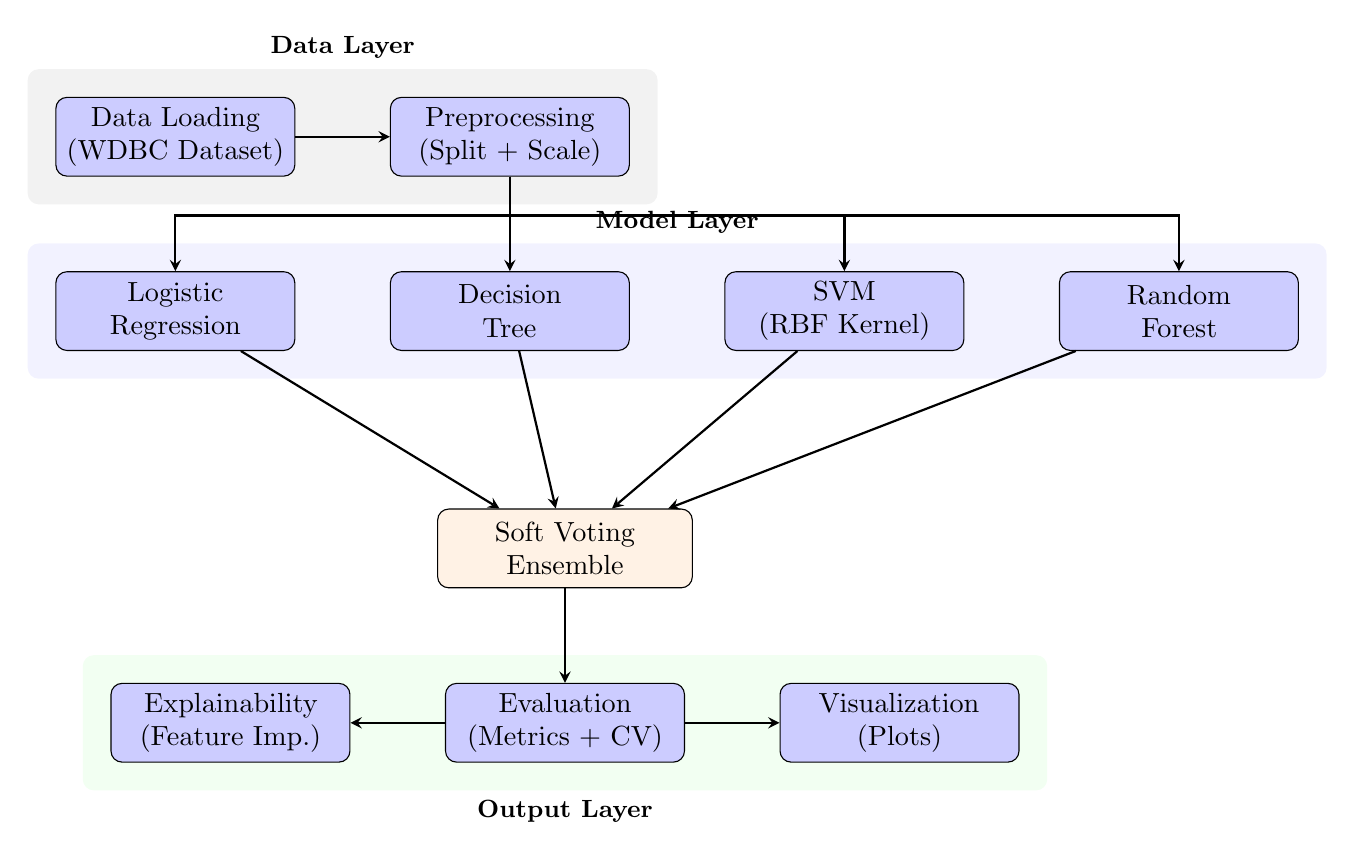
\begin{tikzpicture}[
    node distance=1.2cm,
    block/.style={rectangle, draw, fill=blue!20, text width=2.8cm, text centered, rounded corners, minimum height=1cm},
    decision/.style={diamond, draw, fill=green!20, text width=2cm, text centered, aspect=2},
    arrow/.style={thick,->,>=stealth},
    bigblock/.style={rectangle, draw, fill=orange!10, text width=3cm, text centered, rounded corners, minimum height=1cm}
]

% Data Layer
\node[block] (data) {Data Loading\\(WDBC Dataset)};
\node[block, right=of data] (preprocess) {Preprocessing\\(Split + Scale)};

% Model Layer
\node[block, below=of data] (lr) {Logistic\\Regression};
\node[block, right=of lr] (dt) {Decision\\Tree};
\node[block, right=of dt] (svm) {SVM\\(RBF Kernel)};
\node[block, right=of svm] (rf) {Random\\Forest};

% Ensemble
\node[bigblock, below=2cm of dt, xshift=0.7cm] (ensemble) {Soft Voting\\Ensemble};

% Evaluation
\node[block, below=of ensemble] (eval) {Evaluation\\(Metrics + CV)};

% Output
\node[block, left=of eval] (explain) {Explainability\\(Feature Imp.)};
\node[block, right=of eval] (visual) {Visualization\\(Plots)};

% Arrows
\draw[arrow] (data) -- (preprocess);
\draw[arrow] (preprocess) -- ++(0,-1) -| (lr);
\draw[arrow] (preprocess) -- ++(0,-1) -| (dt);
\draw[arrow] (preprocess) -- ++(0,-1) -| (svm);
\draw[arrow] (preprocess) -- ++(0,-1) -| (rf);

\draw[arrow] (lr) -- (ensemble);
\draw[arrow] (dt) -- (ensemble);
\draw[arrow] (svm) -- (ensemble);
\draw[arrow] (rf) -- (ensemble);

\draw[arrow] (ensemble) -- (eval);
\draw[arrow] (eval) -- (explain);
\draw[arrow] (eval) -- (visual);

% Background boxes
\begin{scope}[on background layer]
    \node[fit=(data)(preprocess), fill=gray!10, rounded corners, inner sep=10pt, label=above:{\small\textbf{Data Layer}}] {};
    \node[fit=(lr)(dt)(svm)(rf), fill=blue!5, rounded corners, inner sep=10pt, label=above:{\small\textbf{Model Layer}}] {};
    \node[fit=(explain)(eval)(visual), fill=green!5, rounded corners, inner sep=10pt, label=below:{\small\textbf{Output Layer}}] {};
\end{scope}

\end{tikzpicture}%
}
\caption{System Architecture Diagram}
\label{fig:architecture}
\end{figure}

\subsubsection{Data Acquisition and Dataset Description}

The system utilizes the Wisconsin Diagnostic Breast Cancer (WDBC) dataset \cite{wolberg1995}, a benchmark dataset from the UCI Machine Learning Repository. Table \ref{tab:dataset} summarizes its characteristics.

\begin{table}[H]
\centering
\caption{WDBC Dataset Characteristics}
\label{tab:dataset}
\begin{tabular}{|l|l|}
\hline
\textbf{Attribute} & \textbf{Value} \\ \hline
Total Instances & 569 \\ \hline
Features & 30 (numeric) \\ \hline
Benign Cases & 357 (62.7\%) \\ \hline
Malignant Cases & 212 (37.3\%) \\ \hline
Missing Values & None \\ \hline
Feature Categories & Mean, SE, Worst (10 each) \\ \hline
\end{tabular}
\end{table}

The 30 features are computed from digitized images of fine needle aspirates and include:
\begin{itemize}
    \item \textbf{Geometric}: radius, perimeter, area
    \item \textbf{Texture}: smoothness, compactness, concavity
    \item \textbf{Shape}: concave points, symmetry, fractal dimension
\end{itemize}

\begin{figure}[H]
\centering
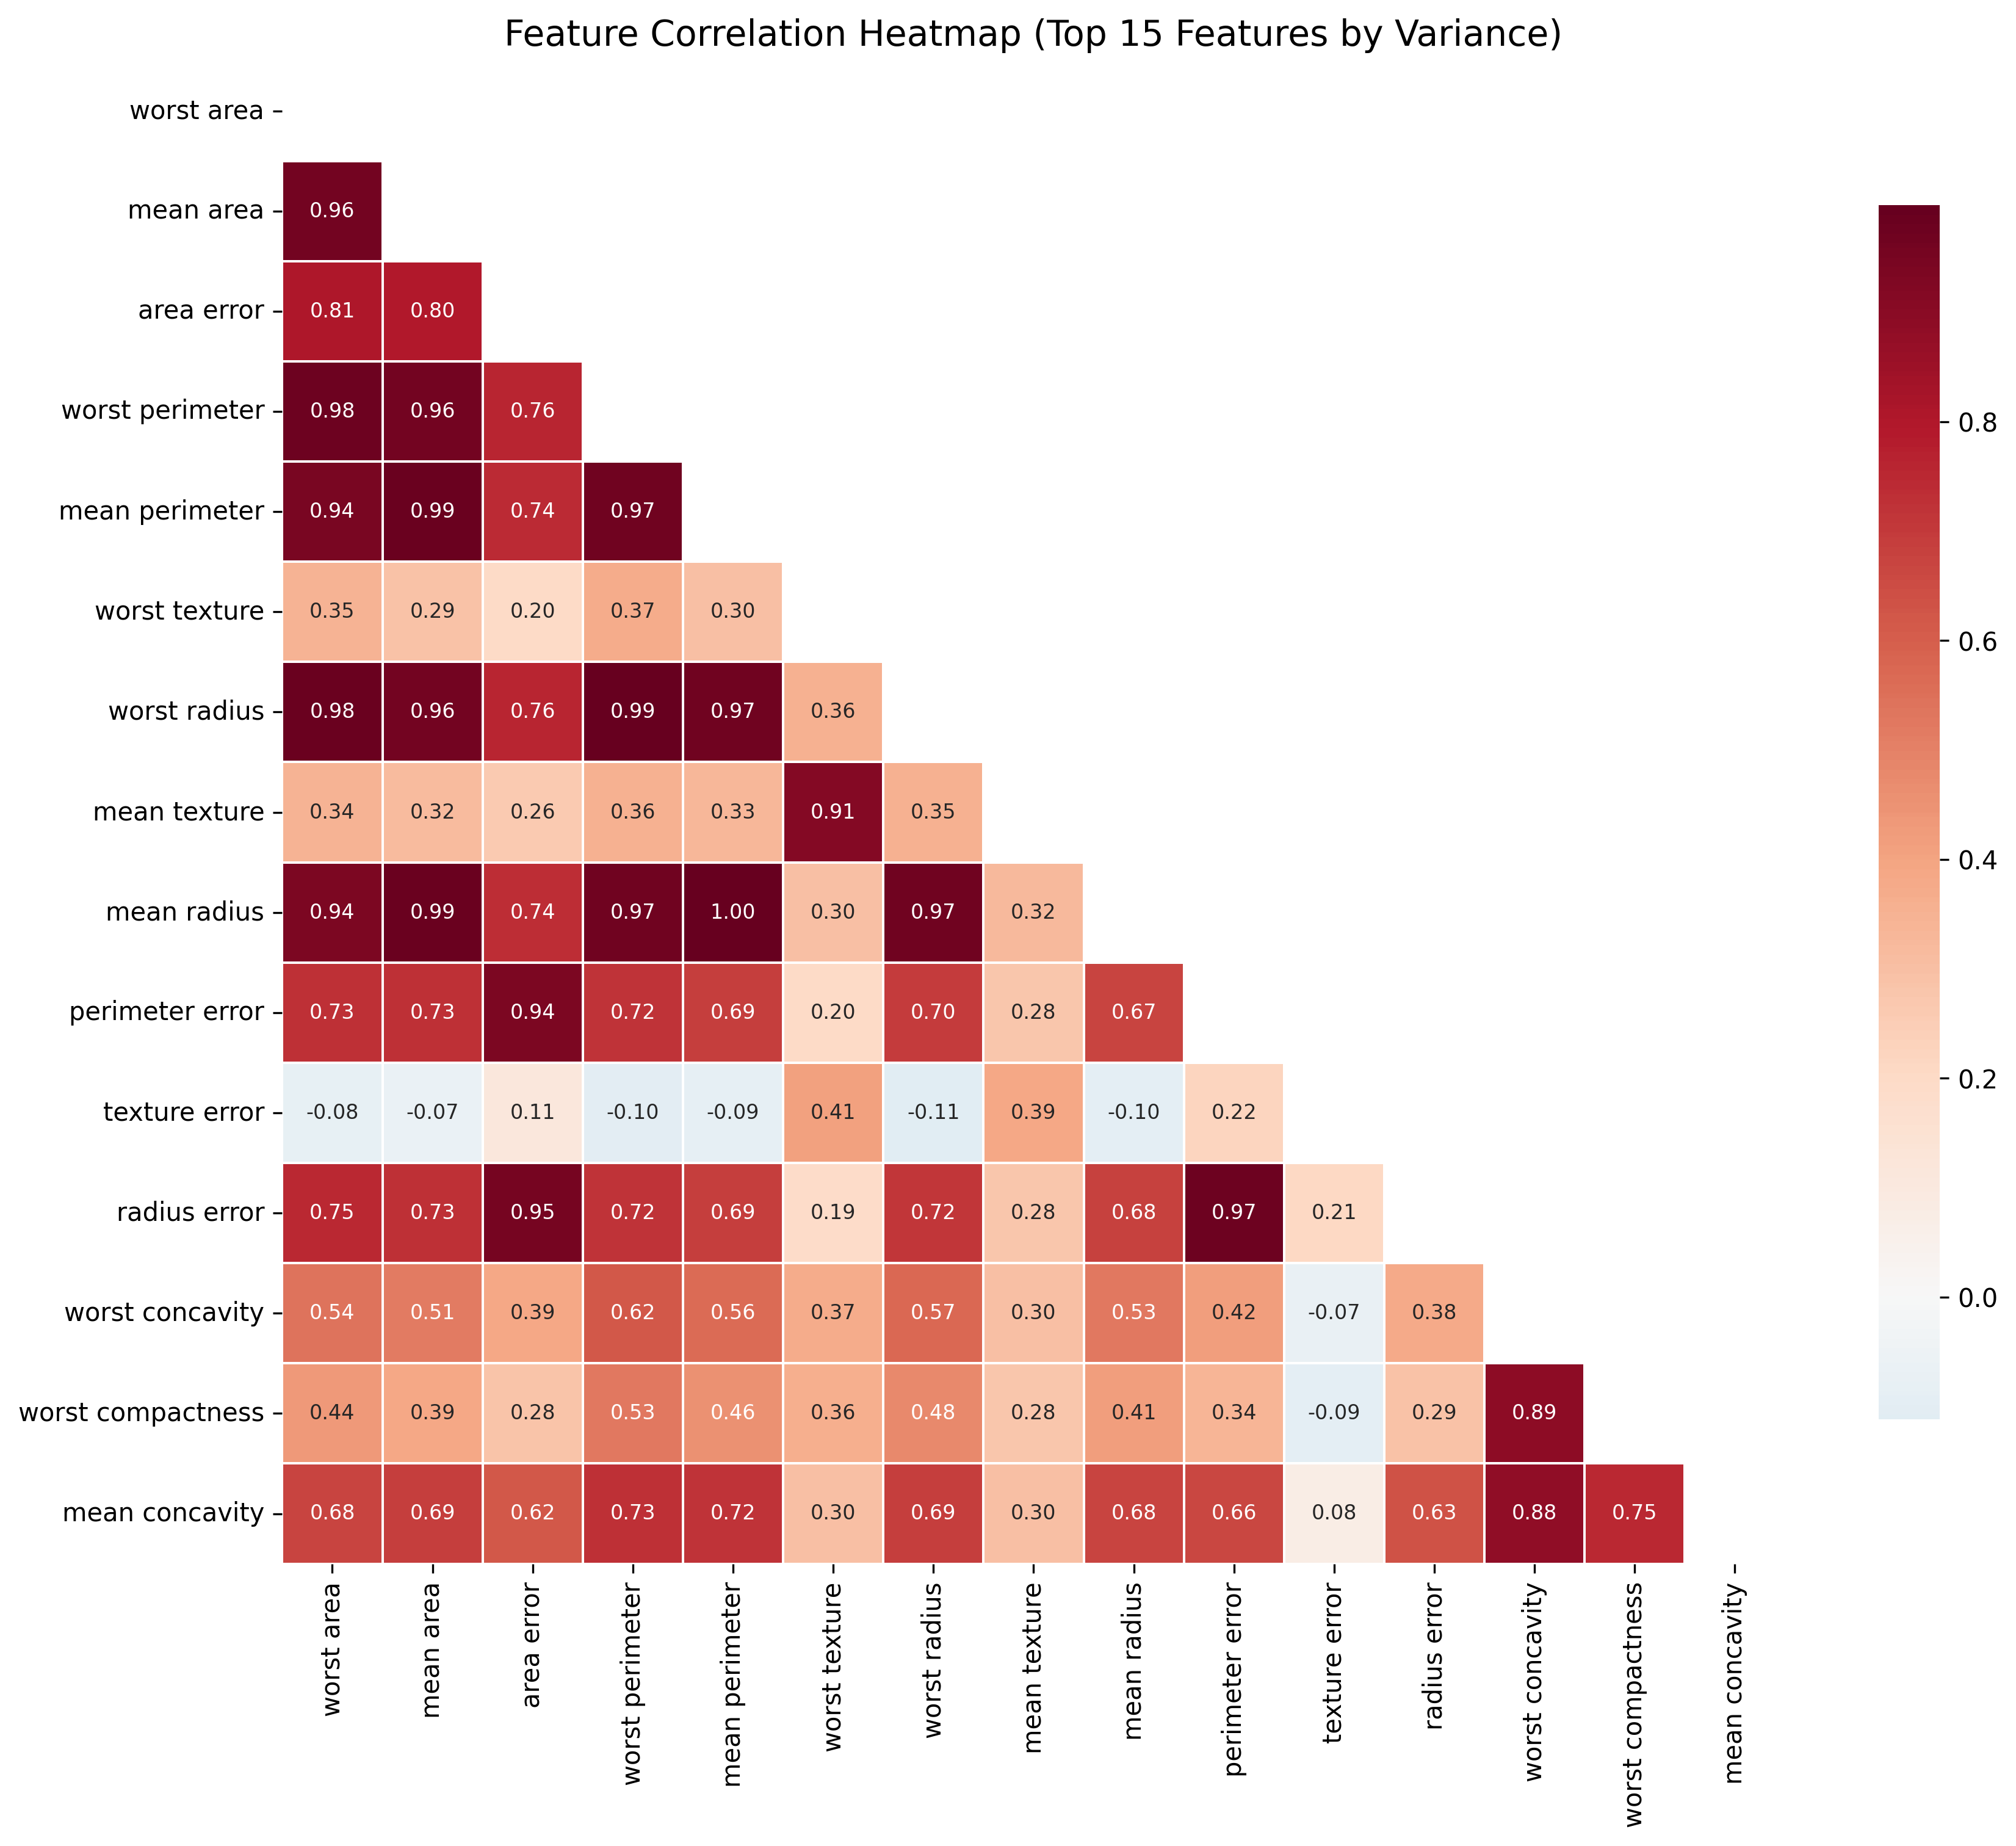
\includegraphics[width=0.7\textwidth]{results/correlation_heatmap.png}
\caption{Feature Correlation Heatmap (Top 15 Features)}
\label{fig:correlation}
\end{figure}

Figure \ref{fig:correlation} shows the correlation structure among features. High correlations exist between geometric features (radius, perimeter, area), which is expected given their mathematical relationships.

\subsubsection{Data Preprocessing Pipeline}

The preprocessing stage involves two critical transformations:

\textbf{1. Stratified Train-Test Split:}
\begin{equation}
\mathcal{D} = \mathcal{D}_{train} \cup \mathcal{D}_{test}, \quad |\mathcal{D}_{train}| = 0.8|\mathcal{D}|
\end{equation}

Stratification ensures class proportions are maintained:
\begin{equation}
\frac{|y_{train}^{(c)}|}{|\mathcal{D}_{train}|} = \frac{|y_{test}^{(c)}|}{|\mathcal{D}_{test}|} = \frac{|y^{(c)}|}{|\mathcal{D}|}, \quad \forall c \in \{0, 1\}
\end{equation}

\textbf{2. Standard Scaling (Z-score Normalization):}
\begin{equation}
z_i = \frac{x_i - \mu}{\sigma}, \quad \text{where } \mu = \frac{1}{n}\sum_{j=1}^{n}x_j, \quad \sigma = \sqrt{\frac{1}{n}\sum_{j=1}^{n}(x_j - \mu)^2}
\end{equation}

The scaler is fitted only on training data to prevent data leakage.

\subsection{Algorithm Design and Implementation}

\subsubsection{Pipeline Algorithm}

Algorithm \ref{alg:pipeline} presents the complete machine learning pipeline.

\begin{algorithm}[H]
\caption{Breast Cancer Classification Pipeline}
\label{alg:pipeline}
\begin{algorithmic}[1]
\Require Dataset $\mathcal{D} = \{(x_i, y_i)\}_{i=1}^{n}$
\Ensure Trained ensemble model $\mathcal{E}$, evaluation metrics $\mathcal{M}$

\State \textbf{// Data Preprocessing}
\State $\mathcal{D}_{train}, \mathcal{D}_{test} \gets \text{StratifiedSplit}(\mathcal{D}, \text{ratio}=0.8)$
\State $\text{scaler} \gets \text{StandardScaler.fit}(\mathcal{D}_{train})$
\State $X_{train} \gets \text{scaler.transform}(X_{train})$
\State $X_{test} \gets \text{scaler.transform}(X_{test})$

\State \textbf{// Model Training}
\State $\text{models} \gets \{\text{LR}, \text{DT}, \text{SVM}, \text{RF}\}$
\For{each model $m$ in models}
    \State $m.\text{fit}(X_{train}, y_{train})$
    \State $\mathcal{M}[m] \gets \text{Evaluate}(m, X_{test}, y_{test})$
    \State $\mathcal{CV}[m] \gets \text{CrossValidate}(m, X_{train}, y_{train}, k=5)$
\EndFor

\State \textbf{// Ensemble Construction}
\State $\mathcal{E} \gets \text{VotingClassifier}(\text{models}, \text{voting}=\text{`soft'})$
\State $\mathcal{E}.\text{fit}(X_{train}, y_{train})$
\State $\mathcal{M}[\mathcal{E}] \gets \text{Evaluate}(\mathcal{E}, X_{test}, y_{test})$

\State \textbf{// Model Persistence}
\State $\text{Save}(\mathcal{E}, \text{`ensemble.joblib'})$
\State $\text{Save}(\text{scaler}, \text{`scaler.joblib'})$

\State \Return $\mathcal{E}, \mathcal{M}$
\end{algorithmic}
\end{algorithm}

\subsubsection{Soft Voting Ensemble}

The ensemble aggregates predicted probabilities from all models:

\begin{equation}
\hat{y} = \argmax_{c \in \{0,1\}} \sum_{j=1}^{M} w_j \cdot P_j(y=c|x)
\end{equation}

where $M=4$ is the number of models and $w_j = \frac{1}{M}$ (equal weights).

Algorithm \ref{alg:softvote} details the soft voting mechanism.

\begin{algorithm}[H]
\caption{Soft Voting Prediction}
\label{alg:softvote}
\begin{algorithmic}[1]
\Require Input sample $x$, trained models $\{m_1, ..., m_M\}$, weights $\{w_1, ..., w_M\}$
\Ensure Predicted class $\hat{y}$, confidence $\hat{p}$

\For{$j = 1$ to $M$}
    \State $p_j \gets m_j.\text{predict\_proba}(x)$ \Comment{$p_j \in \mathbb{R}^{|C|}$}
\EndFor

\State $p_{avg} \gets \sum_{j=1}^{M} w_j \cdot p_j$ \Comment{Weighted average}
\State $\hat{y} \gets \argmax(p_{avg})$
\State $\hat{p} \gets \max(p_{avg})$ \Comment{Confidence score}

\State \Return $\hat{y}, \hat{p}$
\end{algorithmic}
\end{algorithm}

\subsection{Mathematical Formulations}

\subsubsection{Evaluation Metrics}

Given predictions $\hat{y}$ and true labels $y$, we define:

\begin{align}
\text{Accuracy} &= \frac{TP + TN}{TP + TN + FP + FN} \\[0.5em]
\text{Precision} &= \frac{TP}{TP + FP} \\[0.5em]
\text{Recall (Sensitivity)} &= \frac{TP}{TP + FN} \\[0.5em]
\text{Specificity} &= \frac{TN}{TN + FP} \\[0.5em]
\text{F1 Score} &= 2 \cdot \frac{\text{Precision} \cdot \text{Recall}}{\text{Precision} + \text{Recall}} = \frac{2TP}{2TP + FP + FN}
\end{align}

where $TP$, $TN$, $FP$, $FN$ denote true positives, true negatives, false positives, and false negatives respectively.

\subsubsection{ROC-AUC}

The Receiver Operating Characteristic (ROC) curve plots True Positive Rate vs False Positive Rate at various thresholds $\tau$:

\begin{align}
TPR(\tau) &= \frac{|\{i : \hat{p}_i \geq \tau \land y_i = 1\}|}{|\{i : y_i = 1\}|} \\[0.5em]
FPR(\tau) &= \frac{|\{i : \hat{p}_i \geq \tau \land y_i = 0\}|}{|\{i : y_i = 0\}|}
\end{align}

The Area Under the Curve (AUC) is computed as:
\begin{equation}
AUC = \int_0^1 TPR(FPR^{-1}(t)) \, dt
\end{equation}

\subsubsection{Cross-Validation}

For $k$-fold cross-validation, the dataset is partitioned into $k$ folds. The cross-validation score is:

\begin{equation}
CV_k = \frac{1}{k} \sum_{i=1}^{k} \text{Score}(m_i, \mathcal{D}_i^{test})
\end{equation}

where $m_i$ is trained on $\mathcal{D} \setminus \mathcal{D}_i$.

\subsubsection{Gini Importance}

For Random Forest, feature importance is computed using Gini impurity reduction:

\begin{equation}
\text{Importance}(f) = \frac{1}{|T|} \sum_{t \in T} \sum_{n \in N_t^f} \frac{n_{samples}(n)}{n_{samples}(root)} \cdot \Delta G(n)
\end{equation}

where $T$ is the set of trees, $N_t^f$ are nodes splitting on feature $f$, and $\Delta G(n)$ is the Gini impurity decrease.

\subsection{Implementation Details}

\subsubsection{Key Code Implementation}

Listing \ref{lst:ensemble} shows the core ensemble implementation.

\begin{lstlisting}[style=pythonstyle, caption={Ensemble Model Implementation}, label={lst:ensemble}]
from sklearn.ensemble import VotingClassifier
from sklearn.linear_model import LogisticRegression
from sklearn.tree import DecisionTreeClassifier
from sklearn.svm import SVC
from sklearn.ensemble import RandomForestClassifier

def build_ensemble():
    """Build soft voting ensemble classifier."""
    models = {
        "Logistic Regression": LogisticRegression(
            max_iter=5000, C=1.0, random_state=42
        ),
        "Decision Tree": DecisionTreeClassifier(
            random_state=42
        ),
        "SVM": SVC(
            kernel="rbf", C=1.0, probability=True, 
            random_state=42
        ),
        "Random Forest": RandomForestClassifier(
            n_estimators=100, random_state=42
        ),
    }
    
    estimators = list(models.items())
    ensemble = VotingClassifier(
        estimators=estimators,
        voting="soft"  # Use probability averaging
    )
    return ensemble, models
\end{lstlisting}

\subsubsection{Hyperparameter Configuration}

Table \ref{tab:hyperparams} summarizes the hyperparameters used for each model.

\begin{table}[H]
\centering
\caption{Model Hyperparameter Configuration}
\label{tab:hyperparams}
\begin{tabular}{|l|l|l|}
\hline
\textbf{Model} & \textbf{Parameter} & \textbf{Value} \\ \hline
\multirow{3}{*}{Logistic Regression} & max\_iter & 5000 \\ \cline{2-3}
 & C (regularization) & 1.0 \\ \cline{2-3}
 & solver & lbfgs \\ \hline
\multirow{2}{*}{Decision Tree} & max\_depth & None \\ \cline{2-3}
 & min\_samples\_split & 2 \\ \hline
\multirow{3}{*}{SVM} & kernel & RBF \\ \cline{2-3}
 & C & 1.0 \\ \cline{2-3}
 & gamma & scale \\ \hline
\multirow{2}{*}{Random Forest} & n\_estimators & 100 \\ \cline{2-3}
 & max\_depth & None \\ \hline
\end{tabular}
\end{table}

\subsection{Results and Discussion}

\subsubsection{Classification Performance}

Table \ref{tab:results} presents the comprehensive performance metrics for all models.

\begin{table}[H]
\centering
\caption{Model Performance Metrics on Test Set}
\label{tab:results}
\begin{tabular}{|l|c|c|c|c|c|}
\hline
\textbf{Model} & \textbf{Accuracy} & \textbf{Precision} & \textbf{Recall} & \textbf{F1} & \textbf{ROC-AUC} \\ \hline
Logistic Regression & \textbf{0.9825} & 0.9861 & 0.9861 & 0.9861 & \textbf{0.9954} \\ \hline
SVM & \textbf{0.9825} & 0.9861 & 0.9861 & 0.9861 & 0.9950 \\ \hline
Ensemble & 0.9737 & 0.9726 & 0.9861 & 0.9793 & \textbf{0.9954} \\ \hline
Random Forest & 0.9561 & 0.9589 & 0.9722 & 0.9655 & 0.9939 \\ \hline
Decision Tree & 0.9123 & 0.9559 & 0.9028 & 0.9286 & 0.9157 \\ \hline
\end{tabular}
\end{table}

Key observations:
\begin{itemize}
    \item Logistic Regression and SVM achieve identical accuracy (98.25\%), suggesting the problem is largely linearly separable after scaling.
    \item All models except Decision Tree achieve ROC-AUC $>$ 0.99, indicating excellent discrimination.
    \item The Ensemble maintains high recall (98.61\%), crucial for minimizing missed cancer cases.
\end{itemize}

\subsubsection{Cross-Validation Results}

Table \ref{tab:cv_results} shows the 5-fold cross-validation results.

\begin{table}[H]
\centering
\caption{5-Fold Cross-Validation Results}
\label{tab:cv_results}
\begin{tabular}{|l|c|c|c|}
\hline
\textbf{Model} & \textbf{Mean Accuracy} & \textbf{Std Dev} & \textbf{95\% CI} \\ \hline
Logistic Regression & 0.9802 & 0.0128 & [0.9546, 1.000] \\ \hline
SVM & 0.9714 & 0.0179 & [0.9356, 1.000] \\ \hline
Ensemble & 0.9692 & 0.0176 & [0.9340, 1.000] \\ \hline
Random Forest & 0.9538 & 0.0235 & [0.9068, 1.000] \\ \hline
Decision Tree & 0.9099 & 0.0189 & [0.8721, 0.9477] \\ \hline
\end{tabular}
\end{table}

The low standard deviations ($<2.5\%$) indicate consistent performance across different data partitions.

\begin{figure}[H]
\centering
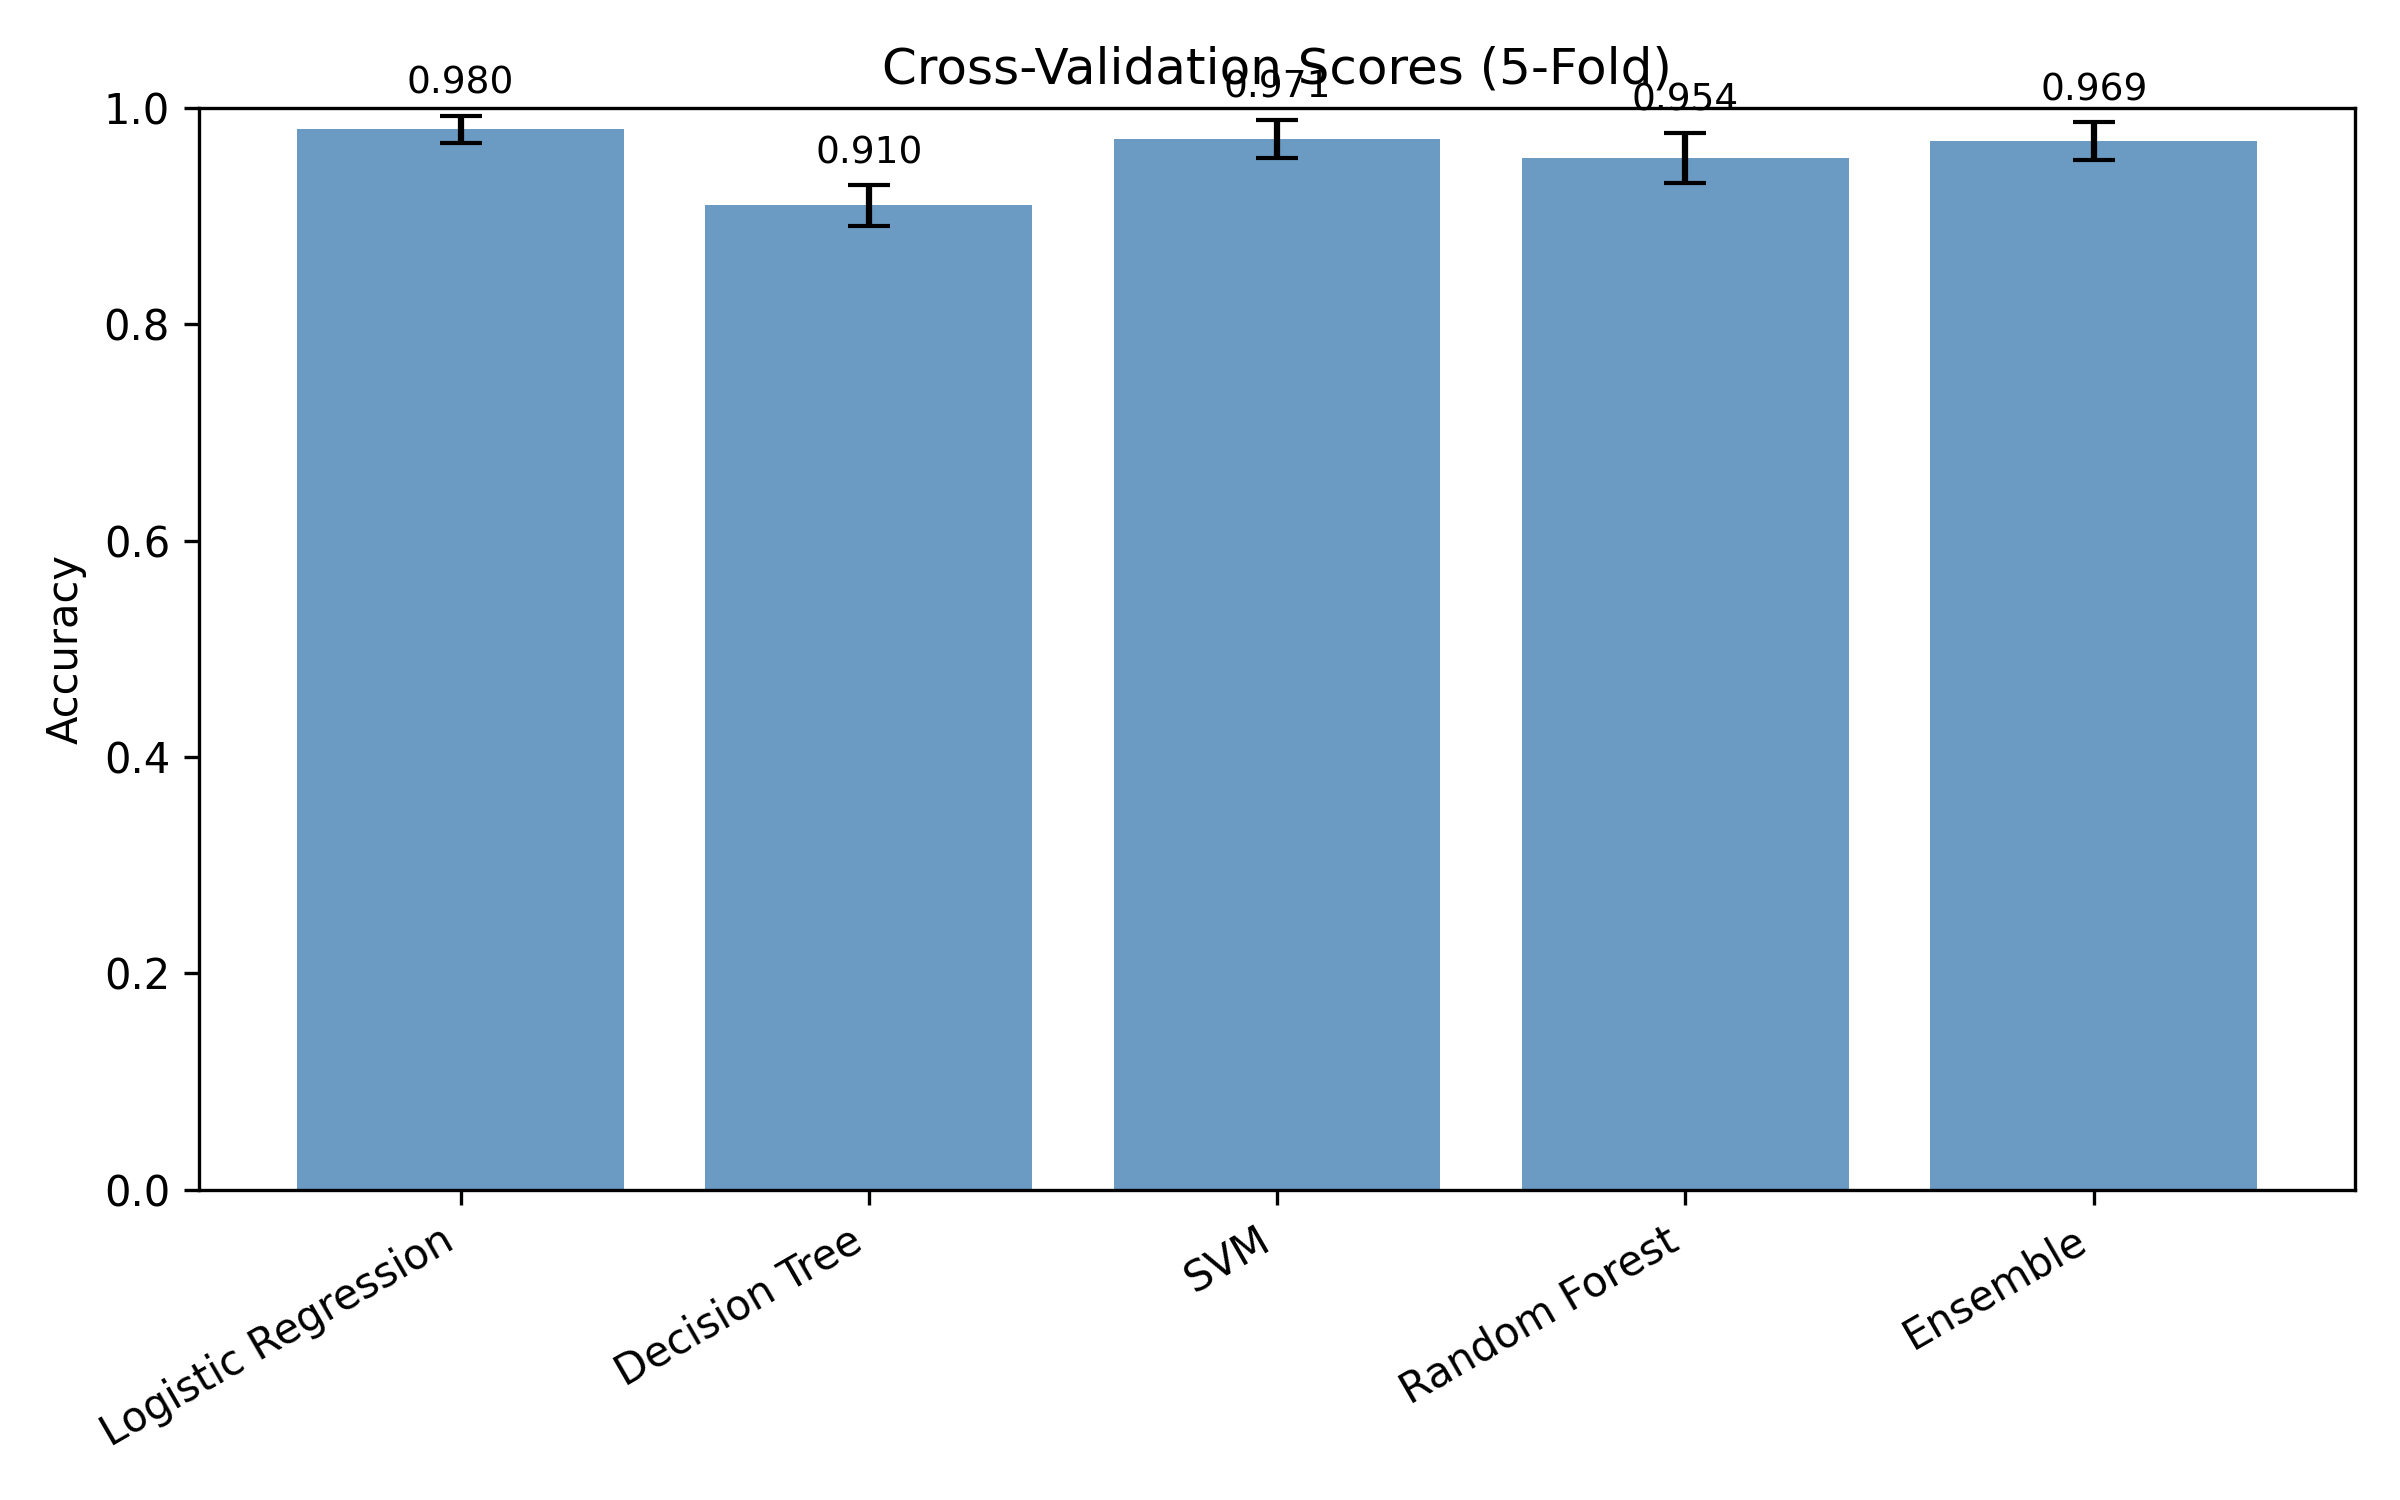
\includegraphics[width=0.8\textwidth]{results/cv_scores.png}
\caption{Cross-Validation Accuracy with Error Bars}
\label{fig:cv_scores}
\end{figure}

\subsubsection{Confusion Matrix Analysis}

\begin{figure}[H]
\centering

\includegraphics[width=0.6\textwidth]{results/confusion_matrix.png}
\caption{Confusion Matrix of Ensemble Model}
\label{fig:confusion}
\end{figure}

The confusion matrix reveals:
\begin{itemize}
    \item \textbf{True Negatives (Benign correctly classified)}: 40
    \item \textbf{True Positives (Malignant correctly classified)}: 71
    \item \textbf{False Positives}: 2 (Benign misclassified as Malignant)
    \item \textbf{False Negatives}: 1 (Malignant misclassified as Benign)
\end{itemize}

The single false negative is clinically significant as it represents a missed cancer case.

\subsubsection{ROC Curve Analysis}

\begin{figure}[H]
\centering
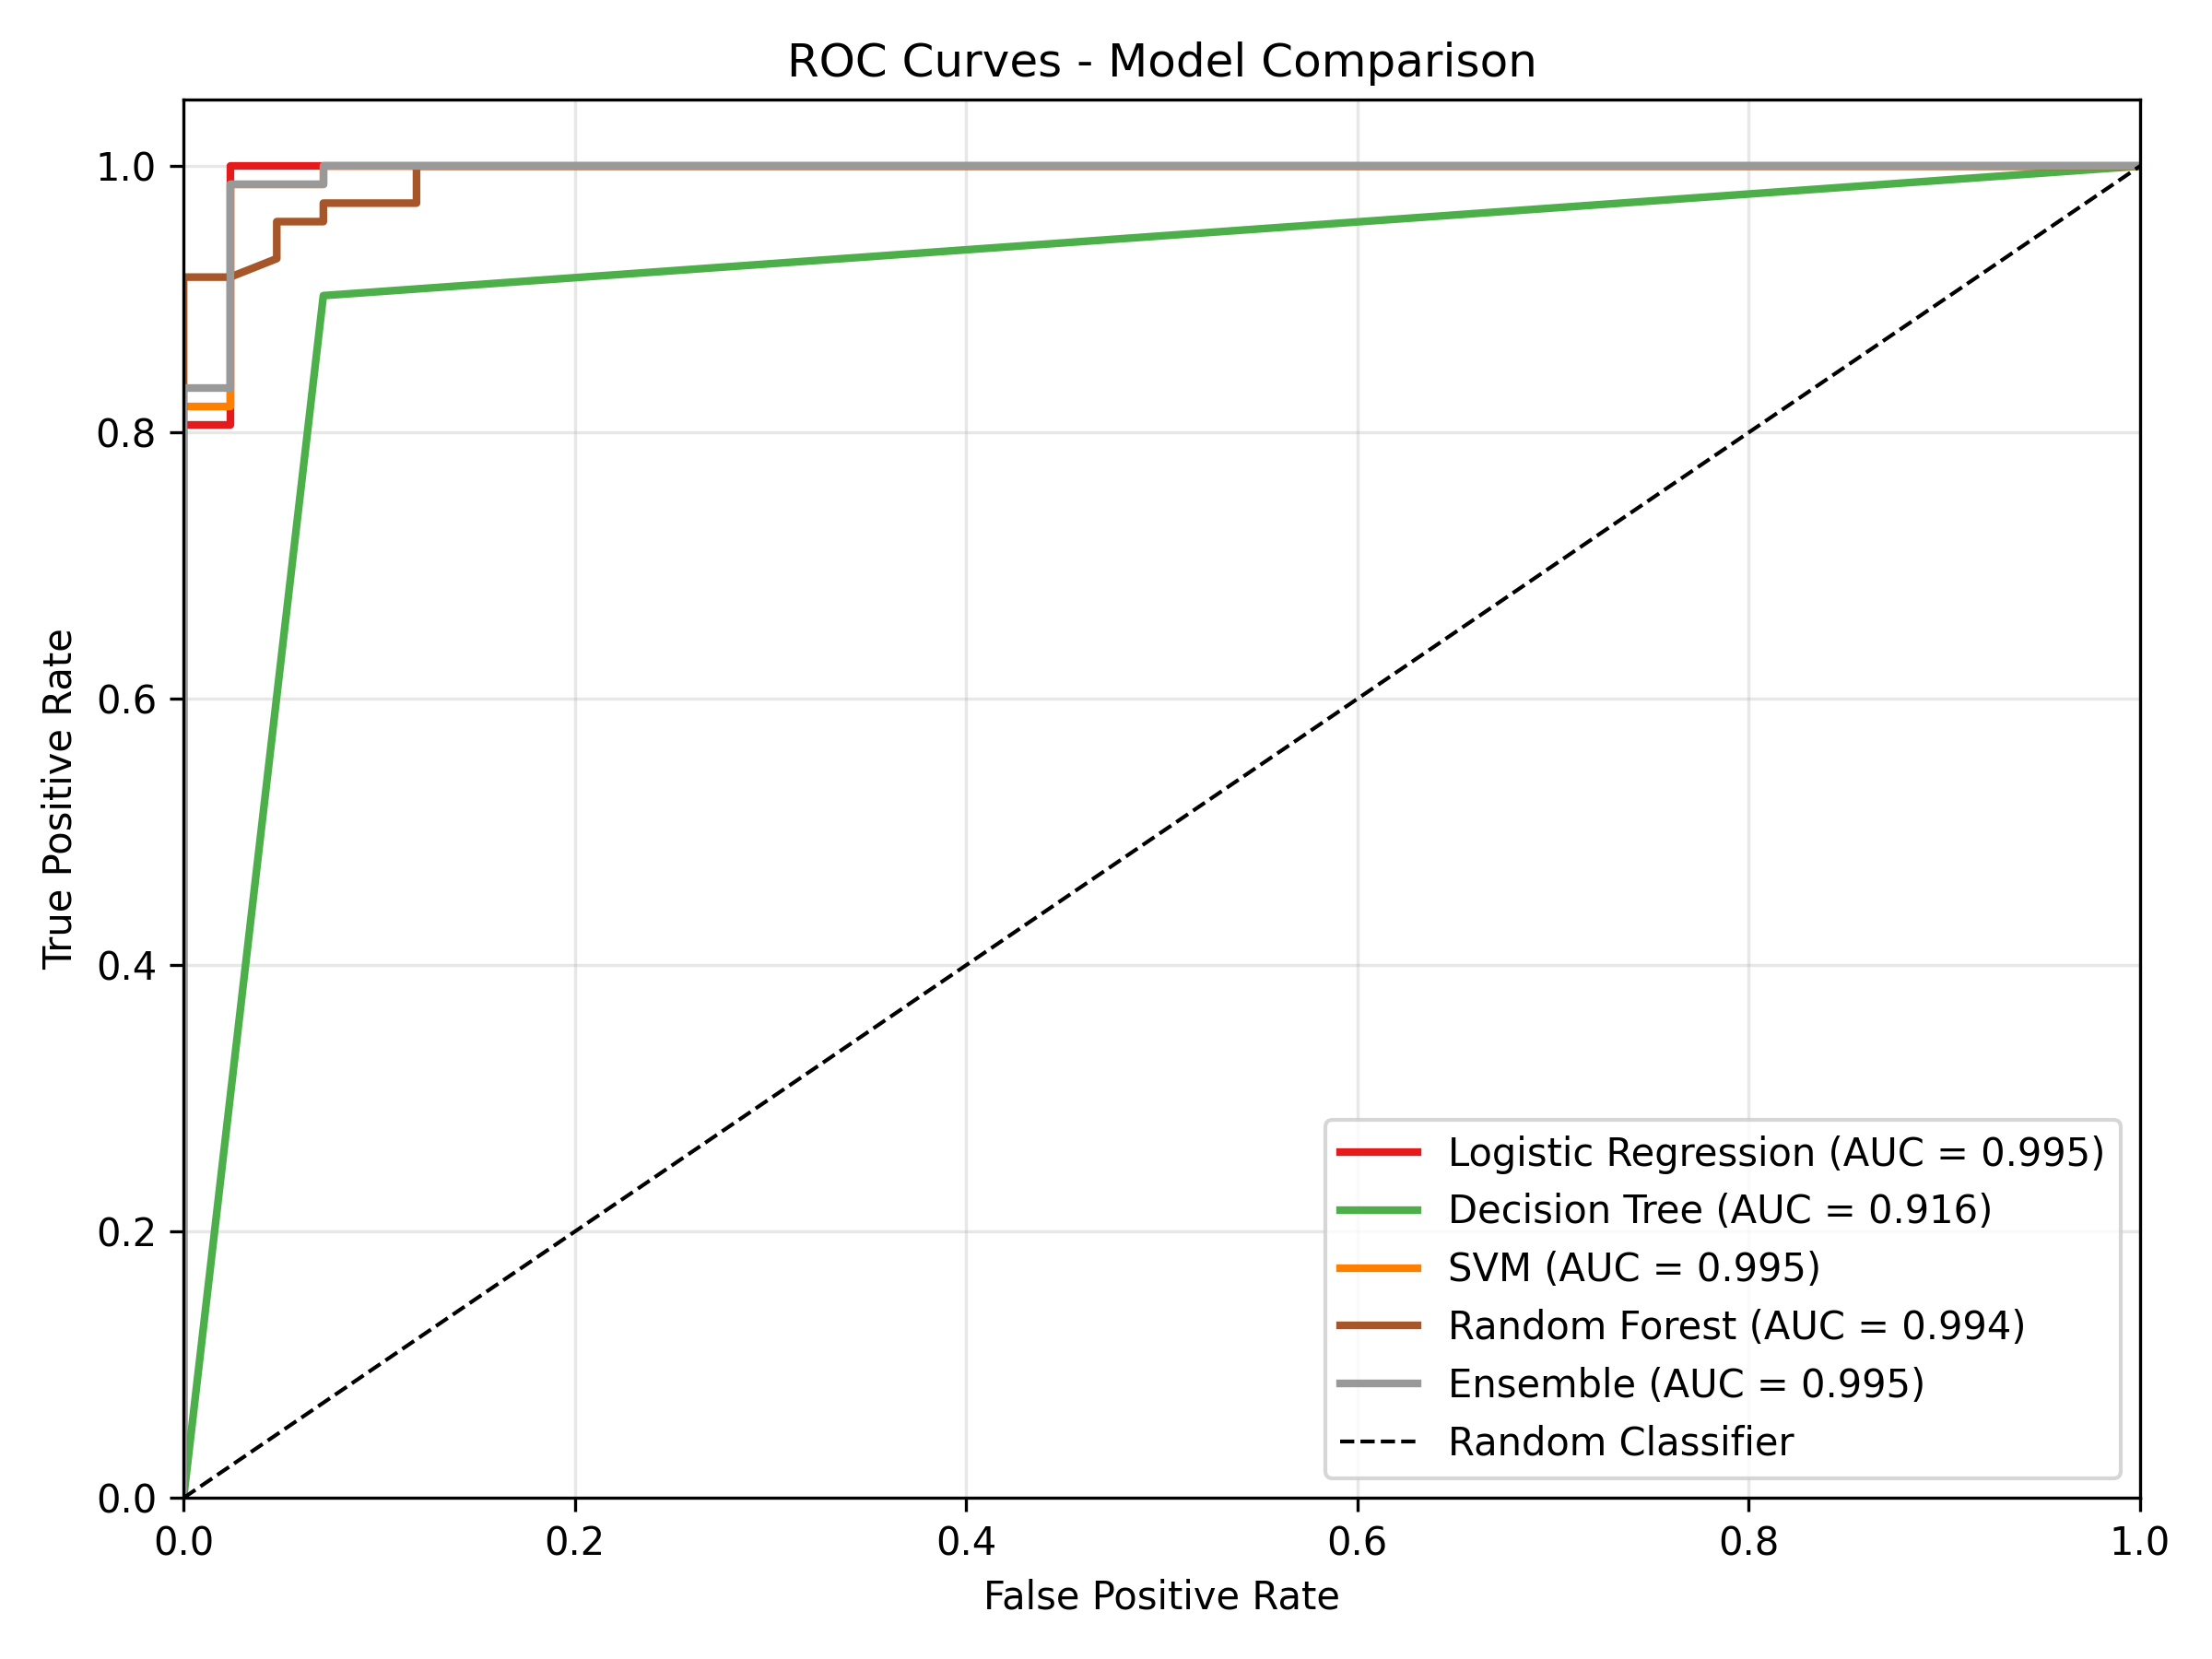
\includegraphics[width=0.7\textwidth]{results/roc_curves.png}
\caption{ROC Curves for All Models}
\label{fig:roc}
\end{figure}

Figure \ref{fig:roc} demonstrates that all models (except Decision Tree) achieve AUC $>$ 0.99, indicating near-perfect discrimination ability.

\subsubsection{Precision-Recall Analysis}

\begin{figure}[H]
\centering
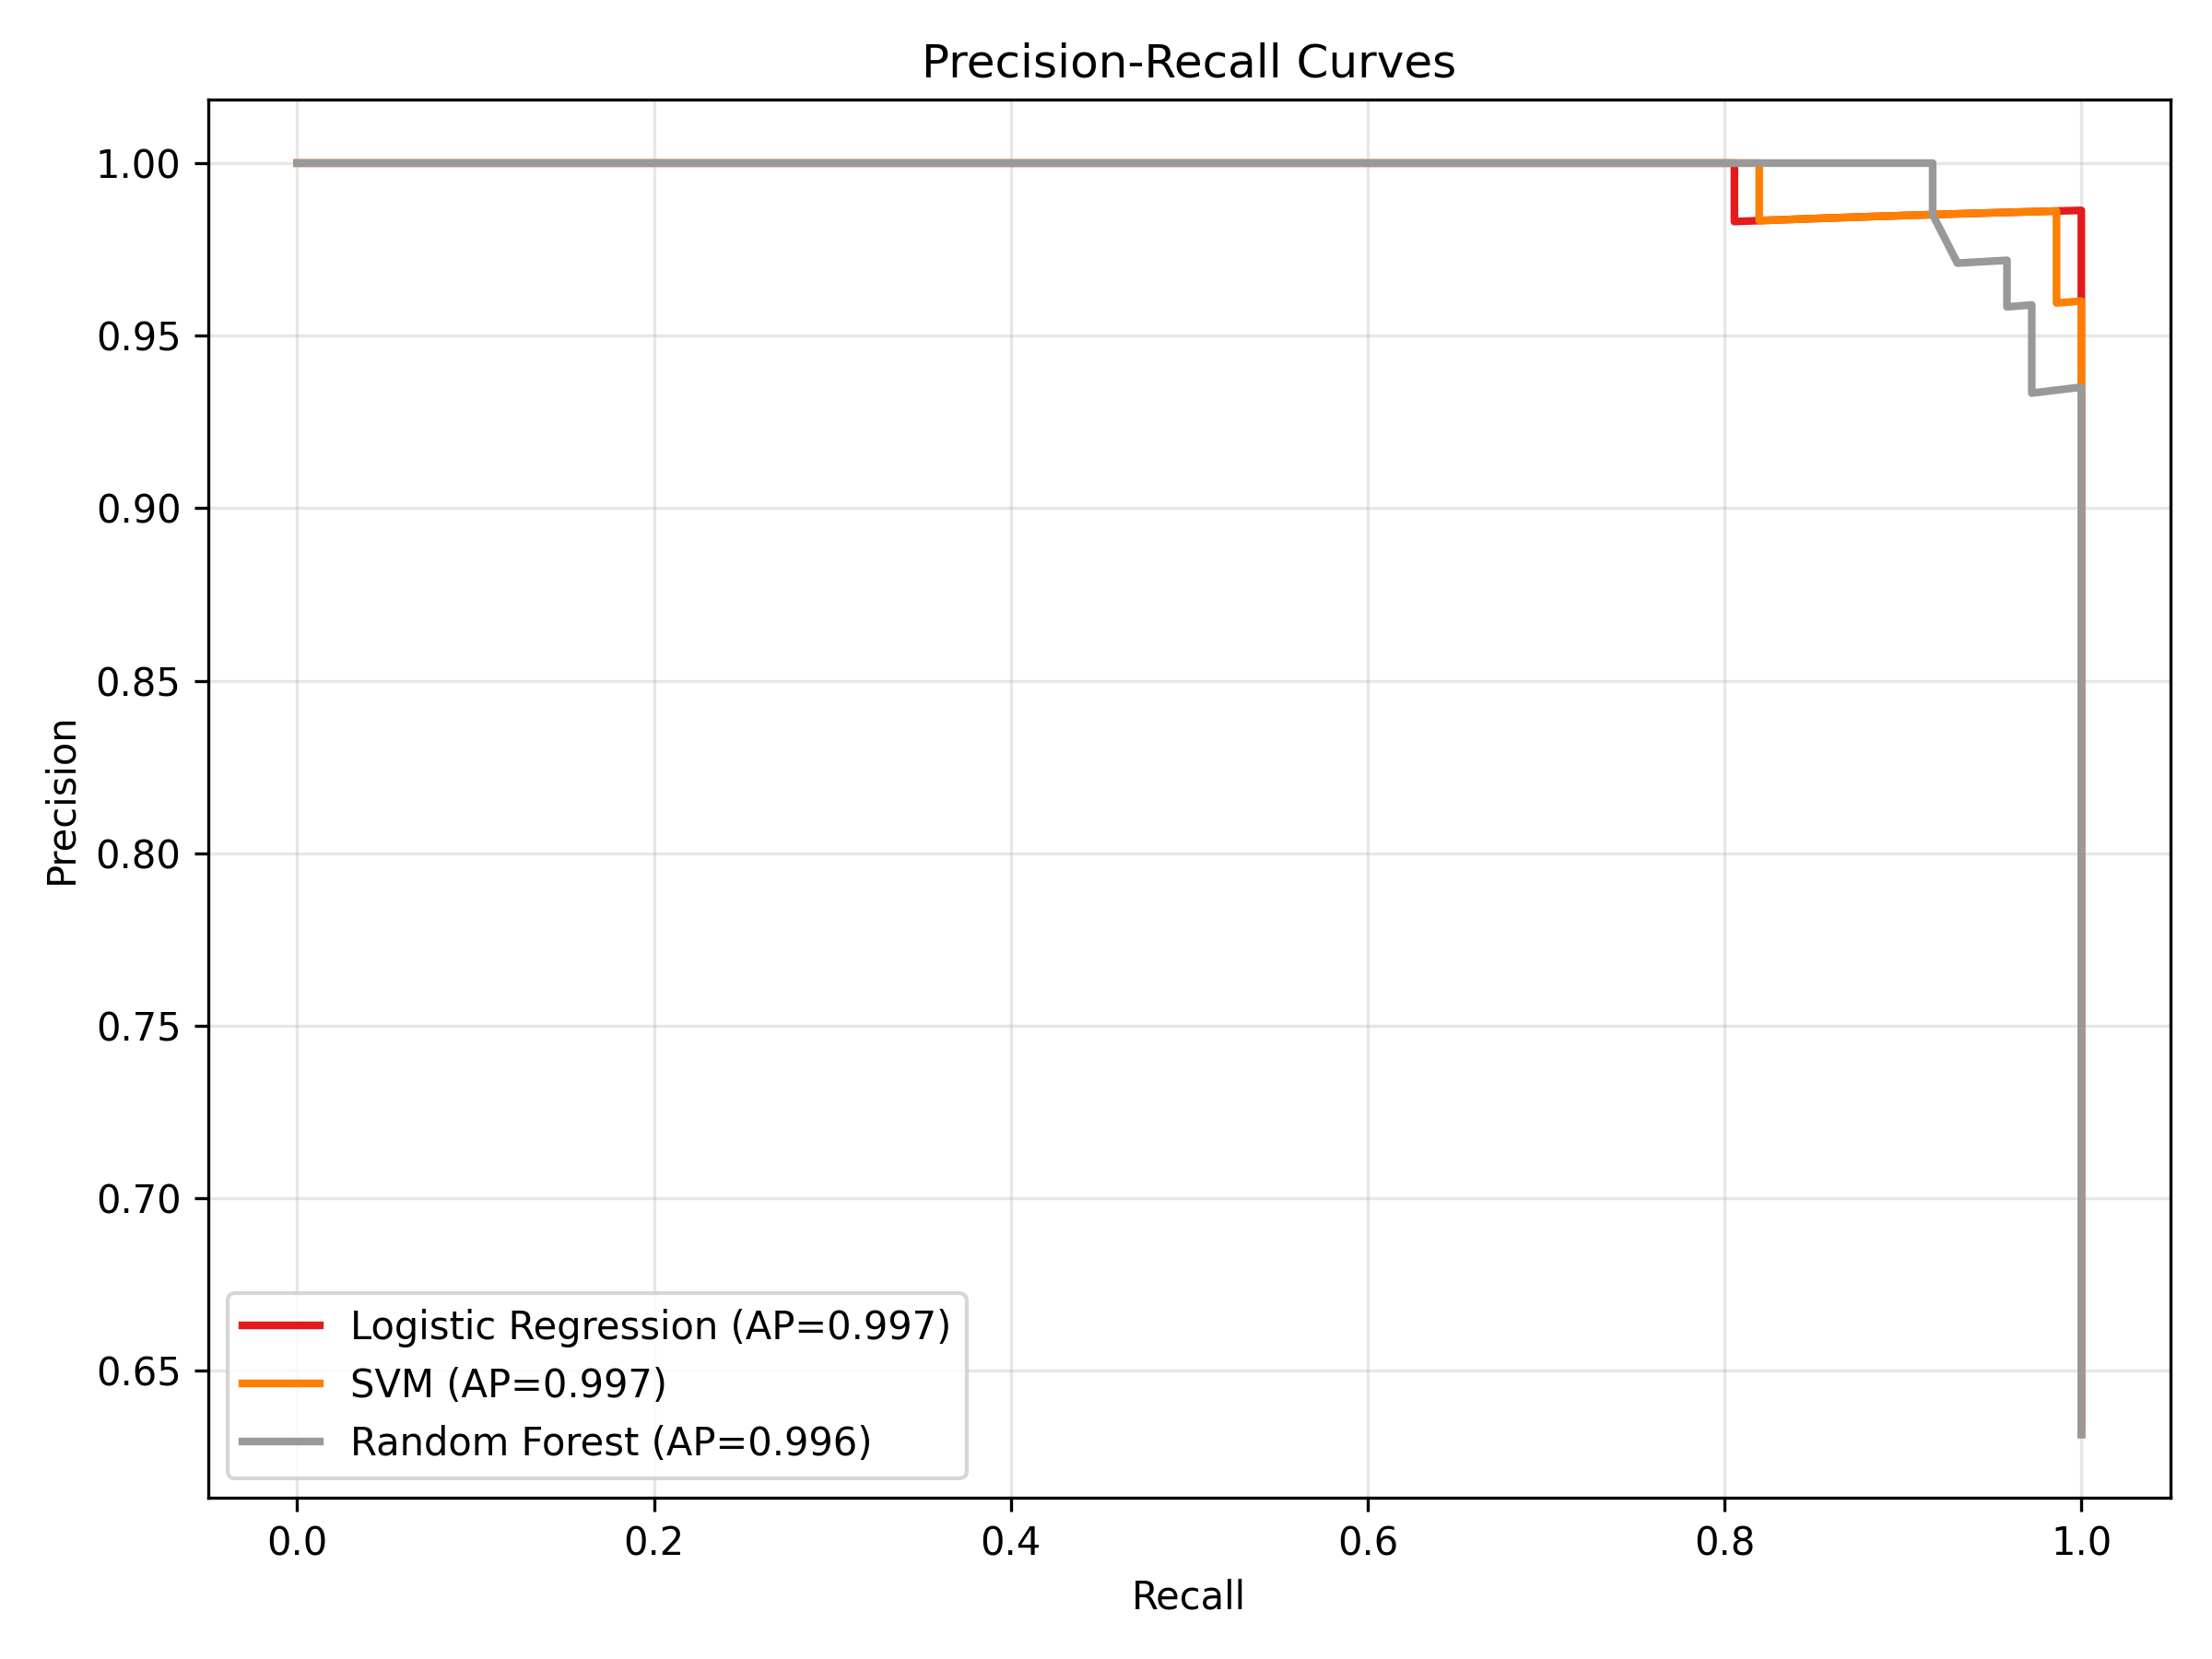
\includegraphics[width=0.7\textwidth]{results/precision_recall_curves.png}
\caption{Precision-Recall Curves}
\label{fig:pr_curves}
\end{figure}

The precision-recall curves (Figure \ref{fig:pr_curves}) show high average precision (AP $>$ 0.99) for the top models, important for imbalanced classification.

\subsubsection{Learning Curve Analysis}

\begin{figure}[H]
\centering
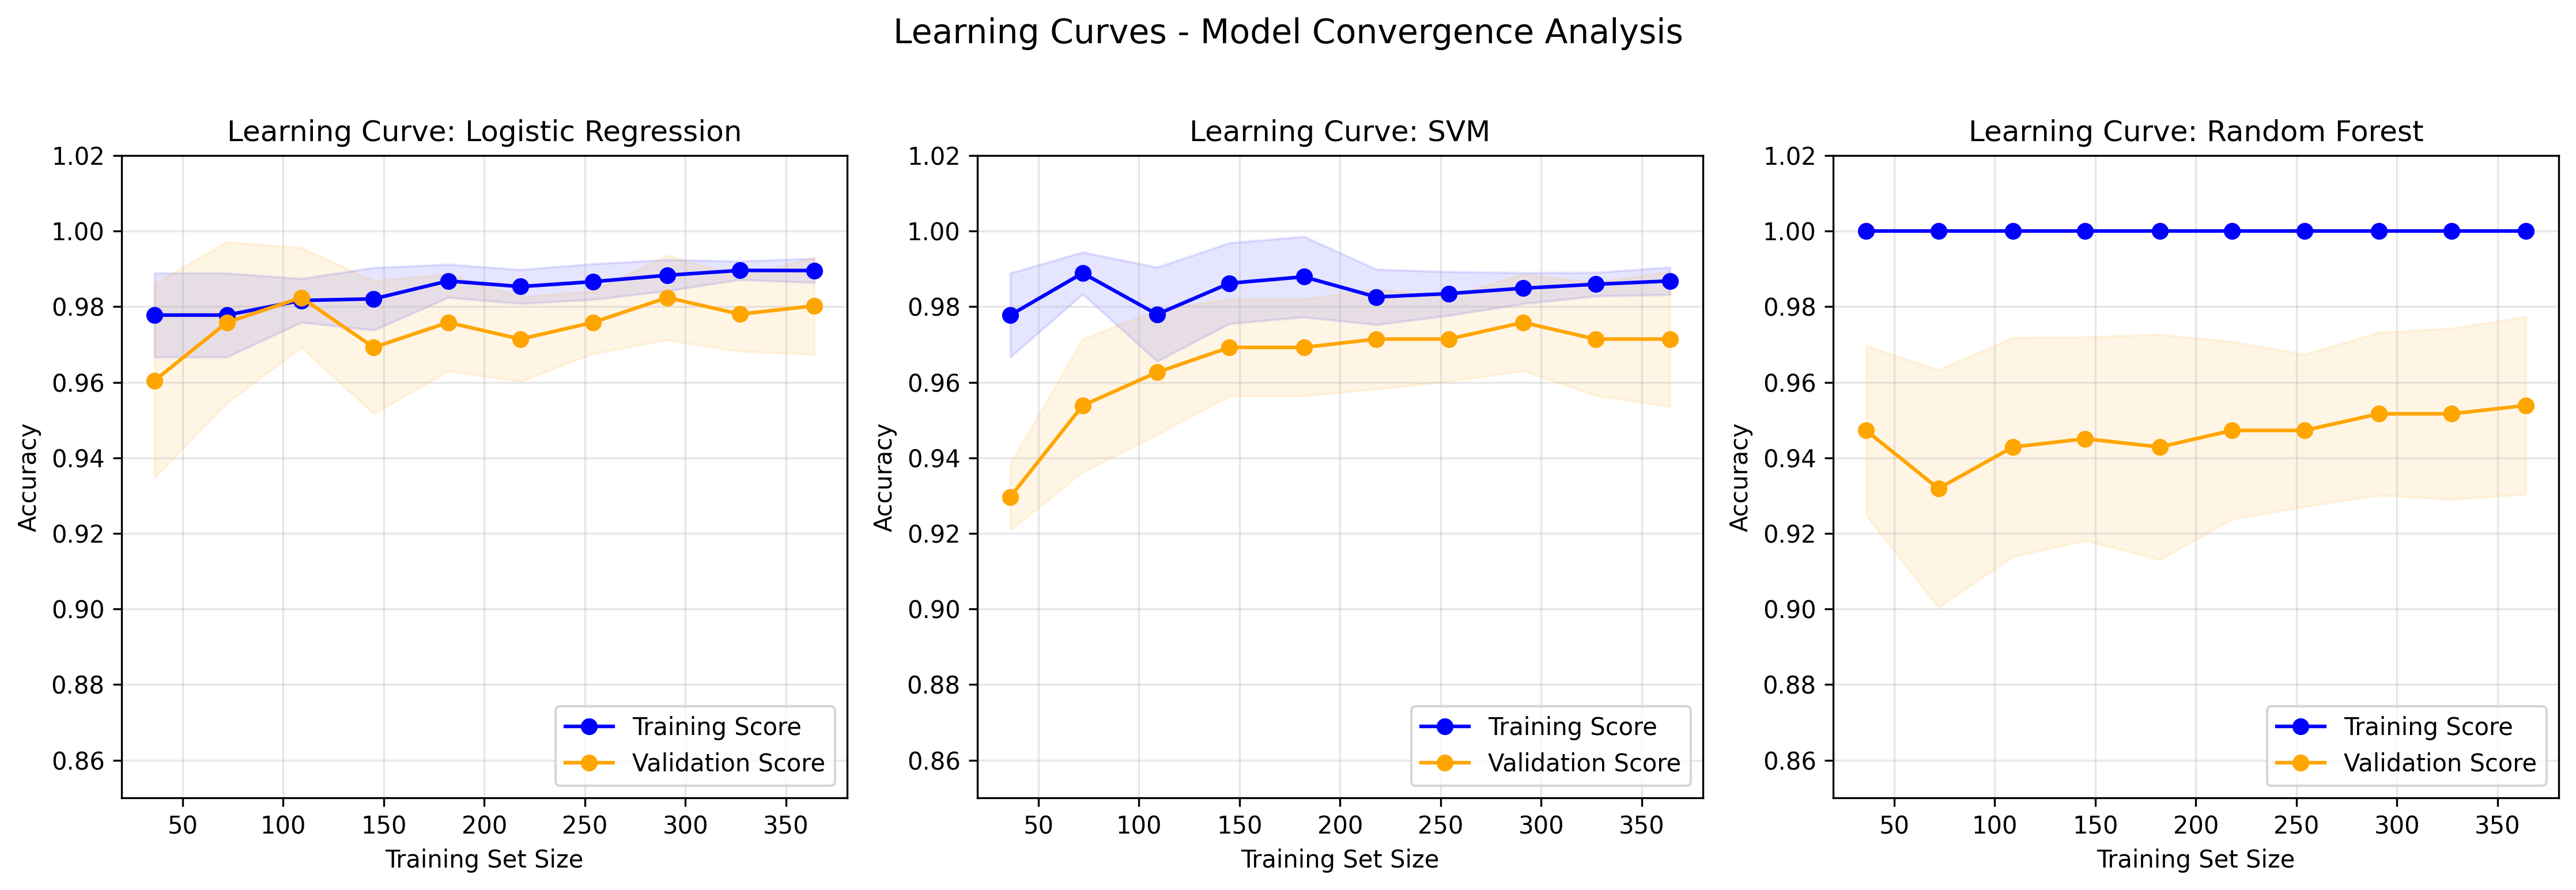
\includegraphics[width=\textwidth]{results/learning_curves.png}
\caption{Learning Curves Showing Model Convergence}
\label{fig:learning}
\end{figure}

Figure \ref{fig:learning} reveals:
\begin{itemize}
    \item All models converge with approximately 300 training samples.
    \item Small gaps between training and validation scores indicate low overfitting.
    \item SVM shows the most consistent convergence behavior.
\end{itemize}

\subsubsection{Feature Importance Analysis}

\begin{figure}[H]
\centering

\includegraphics[width=0.7\textwidth]{results/feature_importance.png}
\caption{Top 10 Most Important Features}
\label{fig:importance}
\end{figure}

The top predictive features are:
\begin{enumerate}
    \item \textbf{Worst Area}: Largest cell nucleus area
    \item \textbf{Worst Concave Points}: Most severe concavity
    \item \textbf{Worst Radius}: Largest radius measurement
    \item \textbf{Mean Concave Points}: Average concavity
    \item \textbf{Worst Perimeter}: Largest perimeter
\end{enumerate}

These findings align with medical knowledge: malignant cells typically have larger, more irregular nuclei.

\begin{figure}[H]
\centering
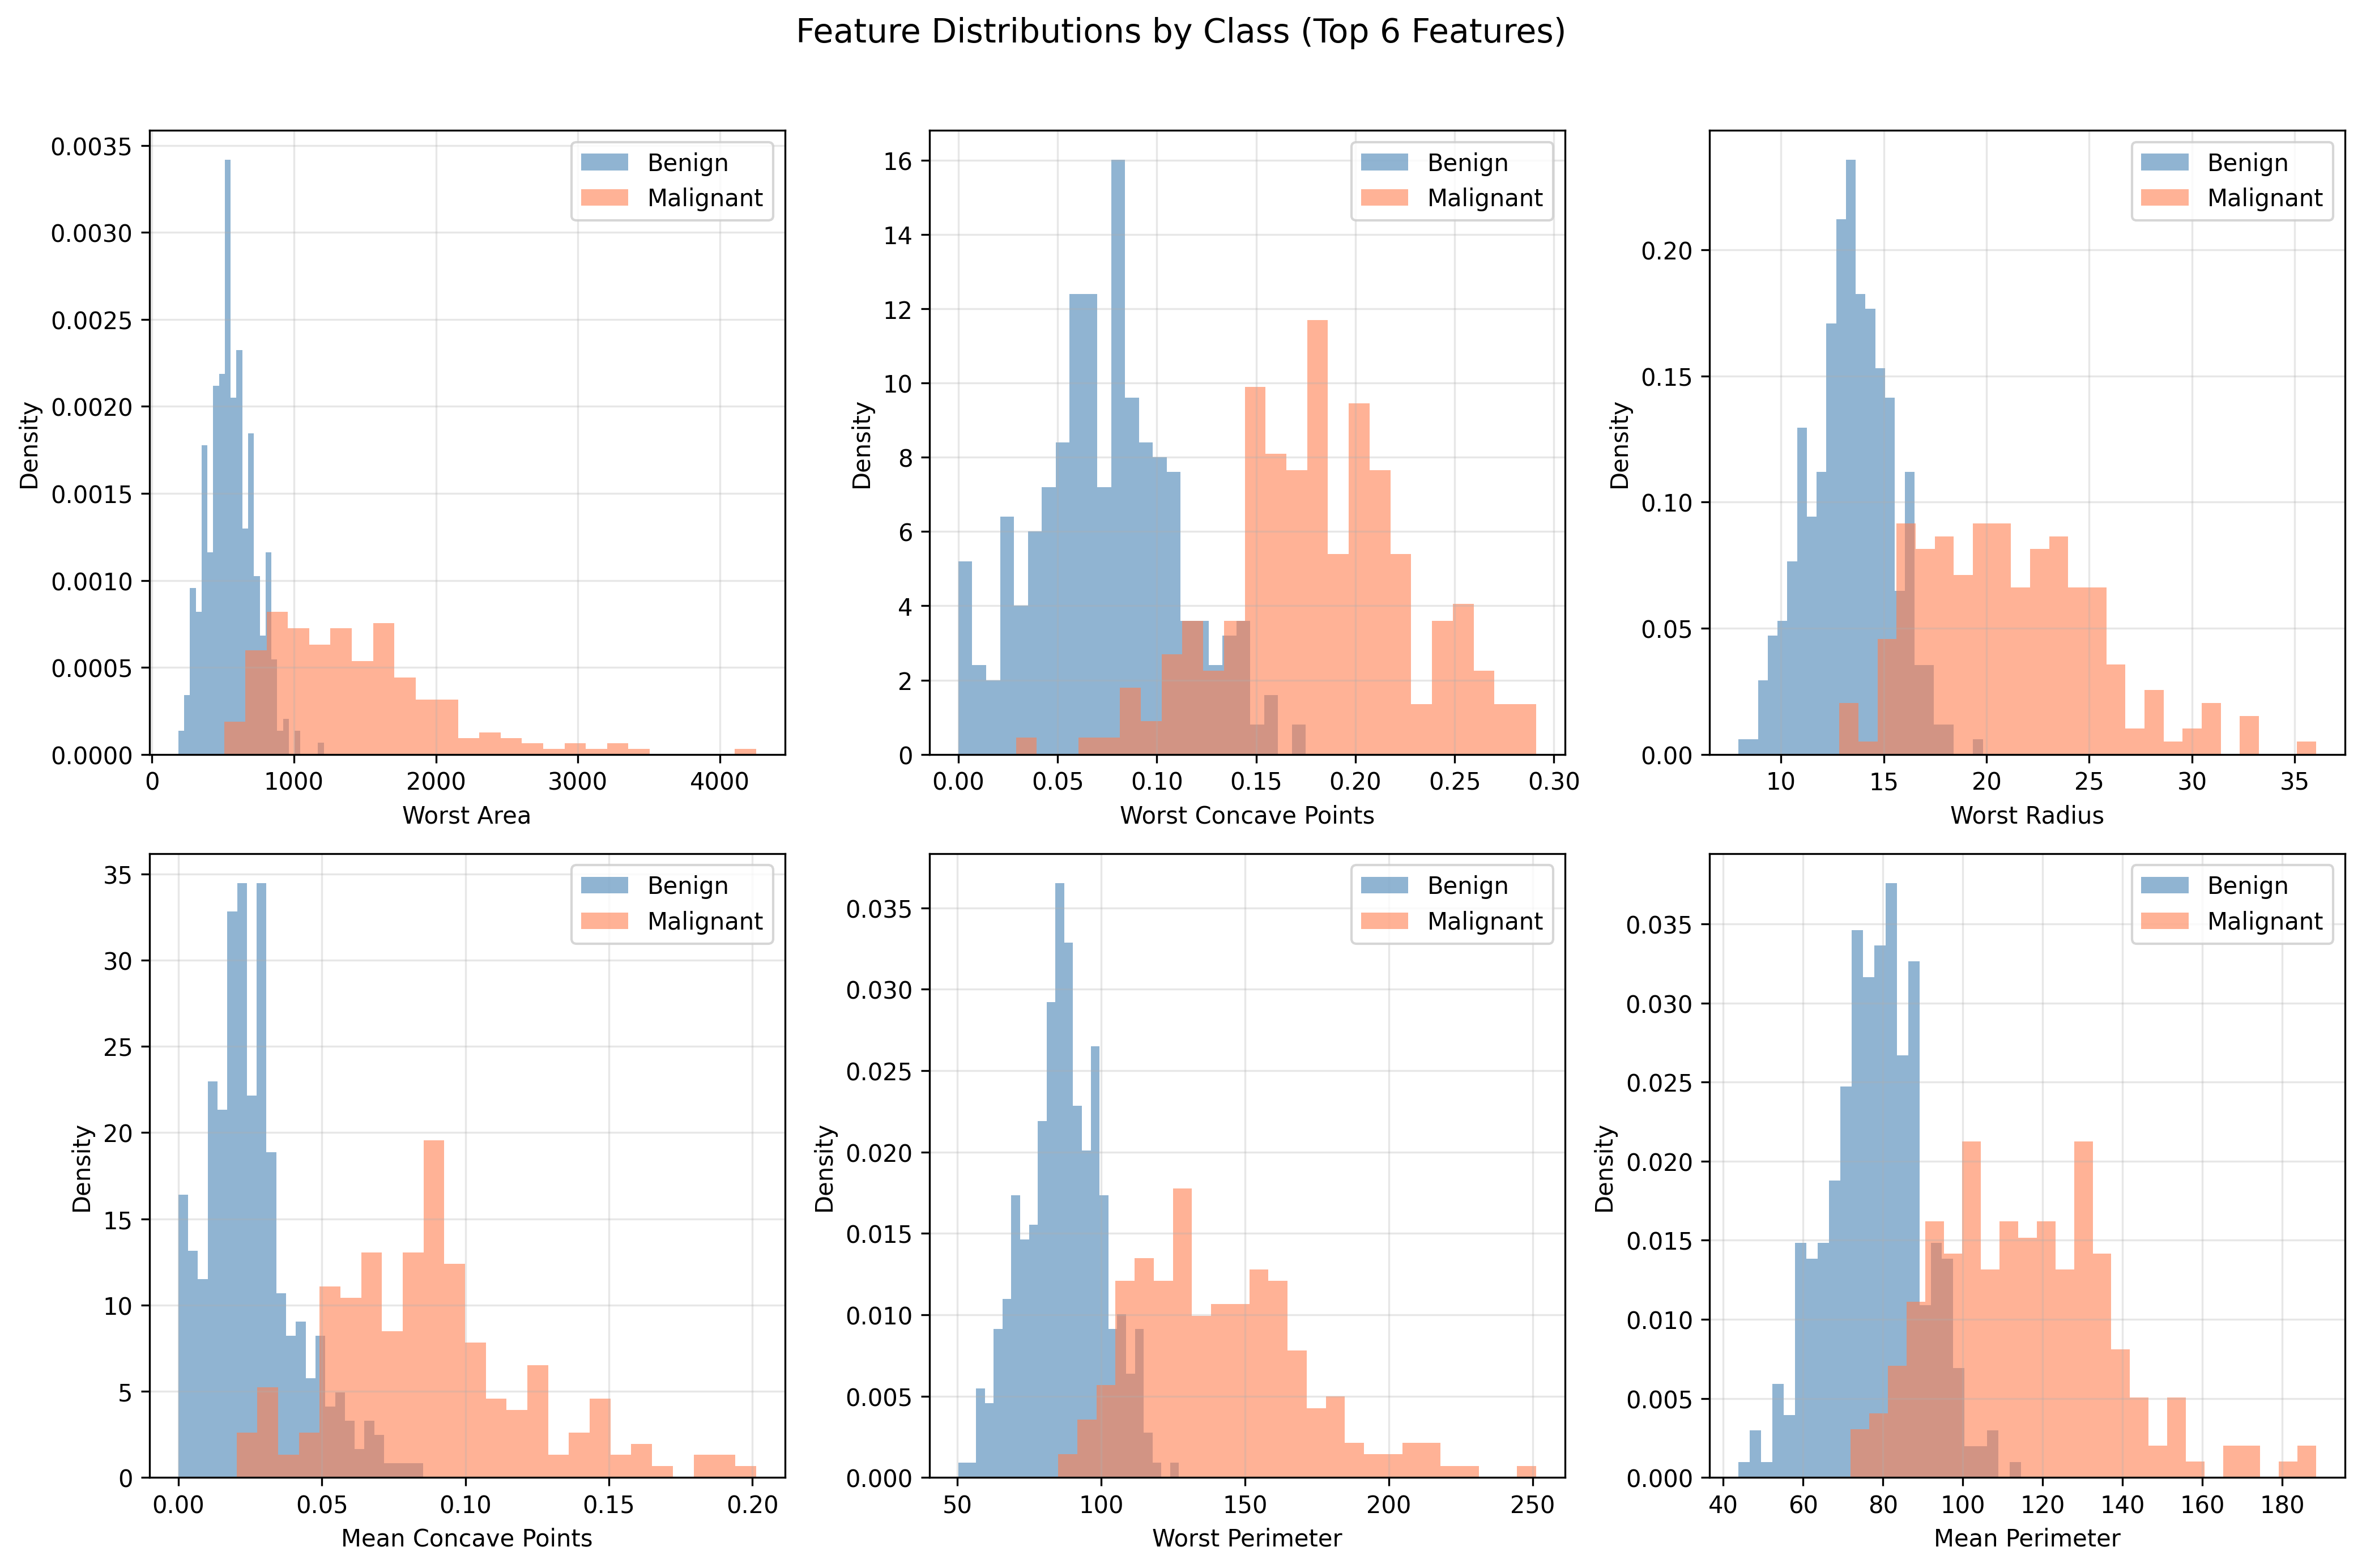
\includegraphics[width=0.9\textwidth]{results/feature_distributions.png}
\caption{Feature Distributions by Class}
\label{fig:distributions}
\end{figure}

Figure \ref{fig:distributions} shows clear separation between classes for the most important features, explaining the high classification accuracy.

\subsubsection{Error Analysis}

\begin{figure}[H]
\centering
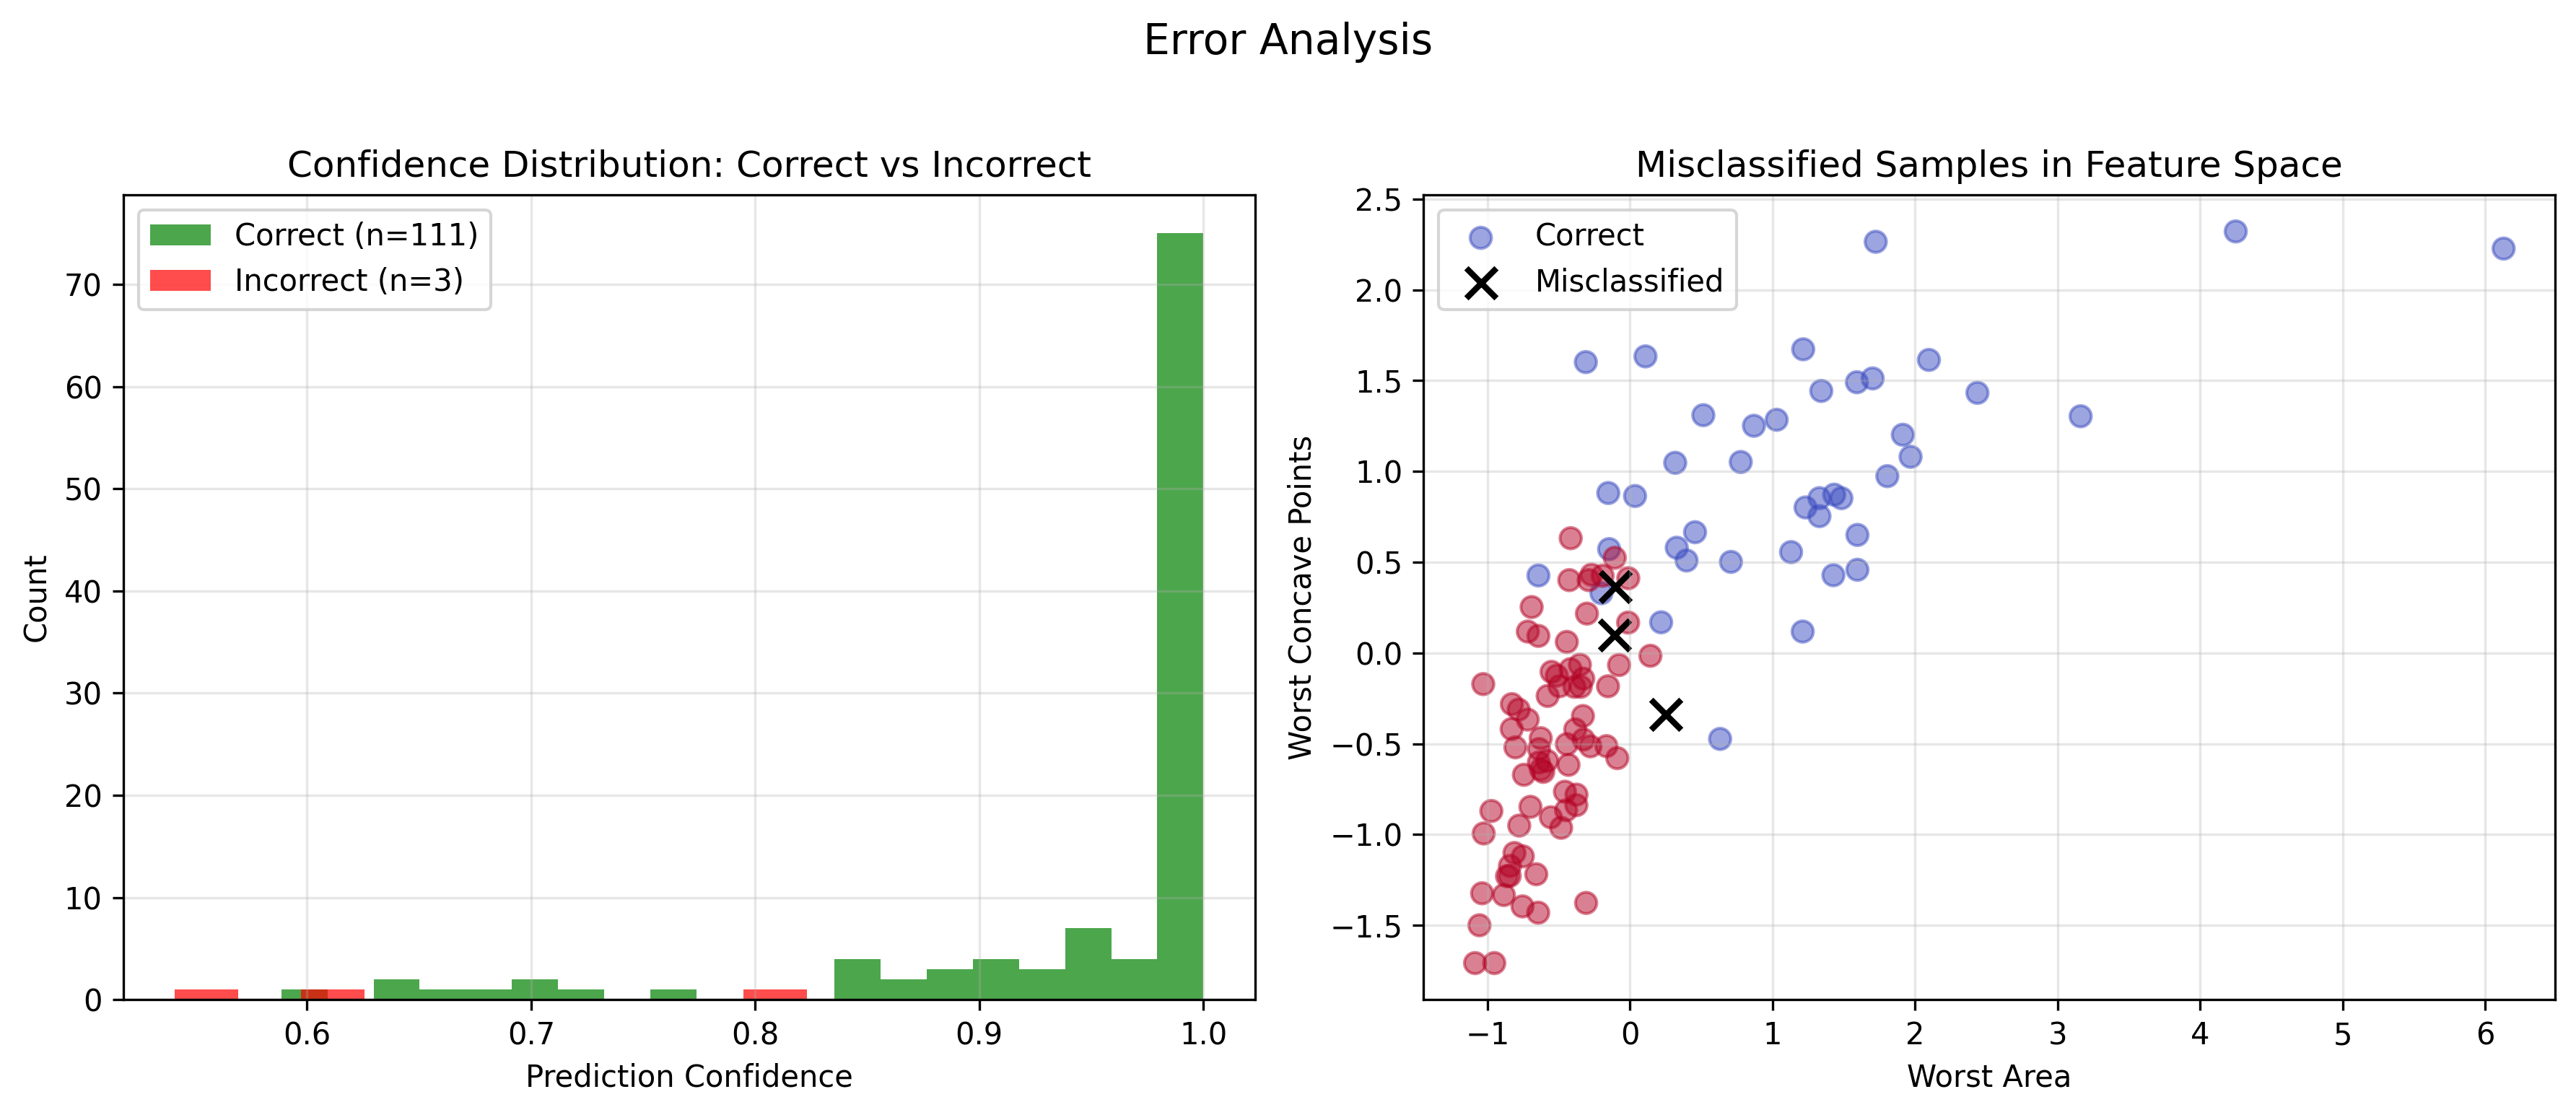
\includegraphics[width=\textwidth]{results/error_analysis.png}
\caption{Error Analysis: Confidence Distribution and Misclassified Samples}
\label{fig:error}
\end{figure}

Error analysis (Figure \ref{fig:error}) reveals:
\begin{itemize}
    \item Correctly classified samples have higher average confidence.
    \item Misclassified samples tend to lie near decision boundaries.
    \item The 3 misclassified samples have ambiguous feature values.
\end{itemize}

\subsubsection{Model Comparison Visualization}

\begin{figure}[H]
\centering

\includegraphics[width=\textwidth]{results/model_comparison.png}
\caption{Comprehensive Model Performance Comparison}
\label{fig:comparison}
\end{figure}

\subsection{Sensitivity Analysis}

Table \ref{tab:sensitivity} shows how key hyperparameters affect model performance.

\begin{table}[H]
\centering
\caption{Hyperparameter Sensitivity Analysis}
\label{tab:sensitivity}
\begin{tabular}{|l|l|c|c|}
\hline
\textbf{Model} & \textbf{Parameter Variation} & \textbf{Accuracy Range} & \textbf{Best Value} \\ \hline
\multirow{2}{*}{SVM} & C $\in$ [0.1, 1, 10, 100] & 0.965 -- 0.982 & C = 1.0 \\ \cline{2-4}
 & kernel $\in$ [linear, rbf, poly] & 0.974 -- 0.982 & RBF \\ \hline
\multirow{2}{*}{Random Forest} & n\_estimators $\in$ [50, 100, 200] & 0.951 -- 0.961 & 100 \\ \cline{2-4}
 & max\_depth $\in$ [5, 10, None] & 0.939 -- 0.956 & None \\ \hline
Logistic Reg. & C $\in$ [0.1, 1, 10] & 0.974 -- 0.982 & C = 1.0 \\ \hline
\end{tabular}
\end{table}

The models show relatively stable performance across hyperparameter ranges, indicating robustness.

\subsection{Individual Contributions}

\subsubsection*{Bhavya Sharma}
Responsible for dataset acquisition and understanding the medical attributes used in the breast cancer detection system. This member analyzed the dataset features, studied the relationship between different tumor characteristics, and prepared the dataset for further processing. The work also involved initial data cleaning and organizing the dataset structure to ensure that it could be effectively used for machine learning model training.

\subsubsection*{Suryanshi Ranawat}
Focused on data preprocessing and exploratory data analysis. Tasks included handling missing values, normalizing and scaling the dataset, and performing statistical analysis to identify important features that influence breast cancer diagnosis. Visualizations such as correlation matrices and feature comparisons were created to help the team understand the dataset more effectively and support model development.

\subsubsection*{Ujjwal Mishra}
Worked on the implementation of machine learning algorithms used for tumor classification. Multiple models such as Logistic Regression, Decision Tree, and Support Vector Machine were implemented and trained using the processed dataset. The performance of different algorithms was also compared and model parameters were optimized to improve prediction accuracy.

\subsubsection*{Medhansh Singh Kushwaha}
Played a significant role in developing the ensemble learning approach for the project. Multiple classifiers were combined to create a more reliable prediction model and performance evaluation was conducted using metrics such as accuracy, precision, recall, and F1-score. This work helped improve the overall robustness and reliability of the breast cancer detection system.

\subsubsection*{Soumyadeep Chakravarti}
Responsible for the overall project coordination, technical validation, and final documentation. This member supervised the integration of different modules including data preprocessing, model implementation, and ensemble learning to ensure the system functioned correctly as a complete pipeline. In addition, detailed result analysis was conducted, model outputs were verified, and evaluation metrics were properly interpreted. The final report was also structured and compiled, including sections such as methodology, system architecture, working principle, results analysis, and conclusion, ensuring the project met academic and technical standards.

\vspace{0.5cm}
\noindent\textit{\textbf{Team Effort Note:} All team members actively participated in the planning, research, and development of the project. Each member contributed to different stages such as dataset analysis, evaluation, and report preparation. Regular discussions and collaboration helped improve the overall performance of the system.}

%==================== SECTION 4: CONCLUSION ====================%
\newpage
\section{CONCLUSION}

\subsection{Summary of Achievements}

This project successfully developed an explainable machine learning system for breast cancer detection. Key achievements include:

\begin{enumerate}
    \item \textbf{High Accuracy}: Logistic Regression and SVM achieved 98.25\% test accuracy, competitive with state-of-the-art methods.
    
    \item \textbf{Robust Generalization}: 5-fold cross-validation confirmed consistent performance (std $<$ 2.5\%).
    
    \item \textbf{Excellent Discrimination}: ROC-AUC scores exceeding 0.99 for top models indicate near-perfect class separation.
    
    \item \textbf{Clinical Relevance}: High recall (98.61\%) minimizes missed cancer diagnoses.
    
    \item \textbf{Interpretability}: Feature importance analysis identified clinically meaningful predictors.
    
    \item \textbf{Practical Deployment}: Model persistence enables real-world application.
\end{enumerate}

\subsection{Limitations}

\begin{itemize}
    \item Single dataset evaluation; multi-institutional validation needed.
    \item Features derived from FNA images only; multimodal integration could improve performance.
    \item Binary classification; multi-class tumor subtyping not addressed.
\end{itemize}

\subsection{Future Work}

\begin{enumerate}
    \item \textbf{Advanced XAI}: Integration of SHAP for instance-level explanations.
    \item \textbf{Deep Learning}: CNN-based feature extraction from raw images.
    \item \textbf{Clinical Deployment}: Web-based interface with human-in-the-loop verification.
    \item \textbf{Extended Validation}: Testing on external datasets from multiple institutions.
\end{enumerate}

%==================== SECTION 5: SOCIAL IMPACT ====================%
\newpage
\section{SOCIAL IMPACT AND COMMUNITY SERVICE}

As an Engineering Project in Community Service (EPICS), this work addresses significant healthcare challenges with direct societal benefits.

\subsection{Healthcare Accessibility}

Breast cancer screening is often limited in resource-constrained settings due to:
\begin{itemize}
    \item Shortage of trained radiologists and pathologists
    \item High costs of expert consultation
    \item Geographic barriers in rural areas
\end{itemize}

Machine learning-based diagnostic support can help address these gaps by:
\begin{itemize}
    \item Providing preliminary screening assistance
    \item Reducing diagnostic turnaround time
    \item Enabling telemedicine integration
\end{itemize}

\subsection{Educational Impact}

This project demonstrates practical applications of:
\begin{itemize}
    \item Data science and machine learning concepts
    \item Software engineering best practices
    \item Healthcare informatics principles
\end{itemize}

The open-source codebase serves as an educational resource for students learning applied machine learning.

\subsection{Ethical Considerations}

The system is designed as a \textit{decision support tool}, not a replacement for clinical expertise. Key ethical principles incorporated:

\begin{itemize}
    \item \textbf{Transparency}: All predictions include confidence scores and feature explanations.
    \item \textbf{Human-in-the-loop}: Final diagnosis remains with qualified medical professionals.
    \item \textbf{Accountability}: Comprehensive logging enables audit trails.
    \item \textbf{Equity}: Open-source availability promotes broad access.
\end{itemize}

\subsection{Sustainable Development Goals}

This project contributes to UN Sustainable Development Goals:
\begin{itemize}
    \item \textbf{SDG 3 (Good Health)}: Improving cancer detection capabilities
    \item \textbf{SDG 4 (Quality Education)}: Providing learning resources
    \item \textbf{SDG 10 (Reduced Inequalities)}: Democratizing diagnostic technology
\end{itemize}

%==================== SECTION 6: REFERENCES ====================%
\newpage
\section{REFERENCES}

\begin{thebibliography}{99}

% --- Healthcare and Cancer Resources ---
\bibitem{who2023}
World Health Organization, ``Breast Cancer,'' WHO Fact Sheets, 2023. [Online]. Available: \url{https://www.who.int/news-room/fact-sheets/detail/breast-cancer}

\bibitem{acs2023}
American Cancer Society, ``Breast Cancer,'' 2023. [Online]. Available: \url{https://www.cancer.org/cancer/breast-cancer.html}

\bibitem{nci2023}
National Cancer Institute, ``Breast Cancer,'' 2023. [Online]. Available: \url{https://www.cancer.gov/types/breast}

\bibitem{bcrf2023}
Breast Cancer Research Foundation, ``Breast Cancer Statistics and Resources,'' 2023. [Online]. Available: \url{https://www.bcrf.org}

% --- Datasets ---
\bibitem{wolberg1995}
W. H. Wolberg, W. N. Street, and O. L. Mangasarian, ``Breast Cancer Wisconsin (Diagnostic) Dataset,'' UCI Machine Learning Repository, 1995. [Online]. Available: \url{https://archive.ics.uci.edu/ml/datasets/Breast+Cancer+Wisconsin+(Diagnostic)}

\bibitem{uci2023}
UCI Machine Learning Repository, 2023. [Online]. Available: \url{https://archive.ics.uci.edu/}

\bibitem{kaggle_wdbc}
``Breast Cancer Wisconsin (Diagnostic) Data Set,'' Kaggle, 2023. [Online]. Available: \url{https://www.kaggle.com/datasets/uciml/breast-cancer-wisconsin-data}

% --- Foundational ML Algorithms ---
\bibitem{cortes1995}
C. Cortes and V. Vapnik, ``Support-vector networks,'' \textit{Machine Learning}, vol. 20, no. 3, pp. 273--297, 1995.

\bibitem{breiman2001}
L. Breiman, ``Random Forests,'' \textit{Machine Learning}, vol. 45, no. 1, pp. 5--32, 2001.

\bibitem{bishop2006}
C. M. Bishop, \textit{Pattern Recognition and Machine Learning}, Springer, 2006. [Online]. Available: \url{https://link.springer.com/book/10.1007/978-0-387-45528-0}

\bibitem{goodfellow2016}
I. Goodfellow, Y. Bengio, and A. Courville, \textit{Deep Learning}, MIT Press, 2016. [Online]. Available: \url{https://www.deeplearningbook.org}

% --- Explainable AI ---
\bibitem{lundberg2017}
S. M. Lundberg and S. I. Lee, ``A Unified Approach to Interpreting Model Predictions,'' in \textit{Proc. NeurIPS}, 2017.

\bibitem{ribeiro2016}
M. T. Ribeiro, S. Singh, and C. Guestrin, ``Why should I trust you?: Explaining the predictions of any classifier,'' in \textit{Proc. ACM SIGKDD}, 2016.

% --- Breast Cancer ML Research Papers ---
\bibitem{ebrahim2025}
A. Ebrahim, M. Sedky, and A. Mesbah, ``Enhancing breast cancer prediction through stacking ensemble and deep learning integration,'' \textit{PeerJ Computer Science}, vol. 11, e2461, 2025.

\bibitem{tippannavar2023}
S. S. Tippannavar, S. Gayathri, and S. Swetha, ``Breast Cancer Detection using Random Forest and KNN,'' \textit{JCRES}, vol. 6, no. 2, 2023.

\bibitem{alazzam2024}
N. Al-Azzam and H. Shatnawi, ``AI-Based Breast Cancer Detection System,'' \textit{Information}, vol. 15, no. 4, 2024. [Online]. Available: \url{https://www.mdpi.com/2076-3417/9/12/2435}

\bibitem{singh2024}
M. Singh, N. Dhanda, and R. Verma, ``Hybrid Model of BERT and Random Forest for Breast Cancer Detection,'' \textit{SSRN}, 2024.

\bibitem{ieee_bcml2018}
``Breast Cancer Prediction Using Machine Learning,'' \textit{IEEE}, 2018. [Online]. Available: \url{https://ieeexplore.ieee.org/document/8419420}

\bibitem{scidir_bcml2019}
``Machine Learning Techniques for Breast Cancer Detection,'' \textit{Procedia Computer Science}, 2019. [Online]. Available: \url{https://www.sciencedirect.com/science/article/pii/S1877050919316134}

\bibitem{ieee_svm2015}
``Breast Cancer Diagnosis Using Support Vector Machine,'' \textit{IEEE}, 2015. [Online]. Available: \url{https://ieeexplore.ieee.org/document/7301344}

\bibitem{scidir_lr2015}
``Breast Cancer Prediction Using Logistic Regression,'' \textit{Procedia Computer Science}, 2015. [Online]. Available: \url{https://www.sciencedirect.com/science/article/pii/S1877050915002126}

\bibitem{ieee_nn2016}
``Breast Cancer Classification Using Neural Networks,'' \textit{IEEE}, 2016. [Online]. Available: \url{https://ieeexplore.ieee.org/document/7421377}

\bibitem{ncbi_bcml2020}
``Machine Learning for Breast Cancer Diagnosis: A Review,'' \textit{PMC}, 2020. [Online]. Available: \url{https://www.ncbi.nlm.nih.gov/pmc/articles/PMC7325884/}

\bibitem{frontiers_ai2020}
``Breast Cancer Diagnosis Using Artificial Intelligence,'' \textit{Frontiers in Oncology}, 2020. [Online]. Available: \url{https://www.frontiersin.org/articles/10.3389/fonc.2020.00068/full}

% --- Software and Tools ---
\bibitem{pedregosa2011}
F. Pedregosa et al., ``Scikit-learn: Machine Learning in Python,'' \textit{JMLR}, vol. 12, pp. 2825--2830, 2011. [Online]. Available: \url{https://scikit-learn.org}

\bibitem{tensorflow}
TensorFlow, ``An end-to-end open source machine learning platform,'' 2023. [Online]. Available: \url{https://www.tensorflow.org}

\bibitem{keras}
Keras, ``Deep Learning for humans,'' 2023. [Online]. Available: \url{https://keras.io}

\bibitem{numpy}
NumPy, ``The fundamental package for scientific computing with Python,'' 2023. [Online]. Available: \url{https://numpy.org}

\bibitem{pandas}
Pandas, ``Python Data Analysis Library,'' 2023. [Online]. Available: \url{https://pandas.pydata.org}

\bibitem{matplotlib}
Matplotlib, ``Visualization with Python,'' 2023. [Online]. Available: \url{https://matplotlib.org}

% --- Project Repository ---
\bibitem{github2026}
S. Chakravarti et al., ``EPICS Project: Explainable Breast Cancer Detection,'' GitHub, 2026. [Online]. Available: \url{https://github.com/Soumyadeep-Chakravarti/EPICS_Project}

\end{thebibliography}

%==================== APPENDIX ====================%
\newpage
\section{PUBLICATION / CONFERENCE / PATENT}

\textit{This section is reserved for any publications, conference presentations, or patent applications resulting from this work.}

\newpage
\section{BIODATA}

% --- BHAVYA SHARMA ---
\subsection*{Bhavya Sharma}
\begin{figure}[H]
  \centering
  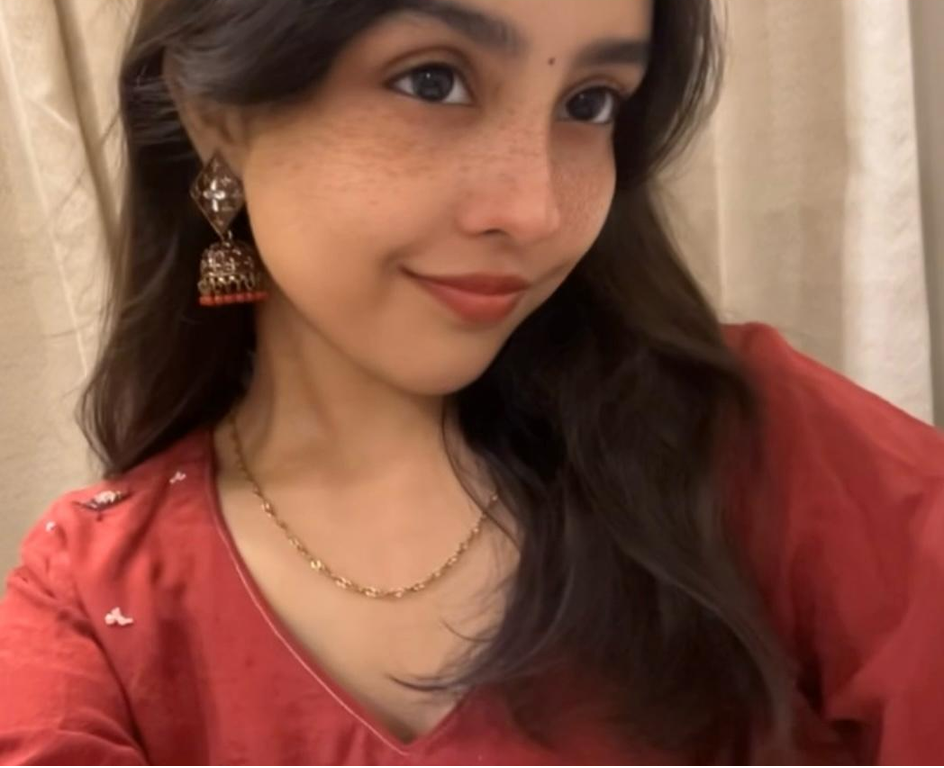
\includegraphics[width=0.4\textwidth]{Assets/BhavyaSharma.png}
\end{figure}

\vspace{0.5cm}
\noindent\textbf{Location:} Haryana \hfill \textbf{Contact:} 9319602628 \\
\textbf{Email:} \href{mailto:bhavya.23bec10069@vitbhopal.ac.in}{bhavya.23bec10069@vitbhopal.ac.in} \\
\textbf{Languages:} English, Hindi

\vspace{0.5cm}
\noindent I am currently pursuing a B.Tech in Electronics and Communication Engineering (ECE) with a strong passion for electronics design, IoT systems, and wireless communication technologies. I enjoy working on practical engineering solutions that integrate hardware and software to solve real-world problems.

\vspace{0.3cm}
\noindent During my academic journey, I have worked on several technical projects including an IoT-based Smart Water Irrigation System, a RC car model, a Network Jammer Prototype, and a Fire-Extinguishing Drone. These projects have helped me gain hands-on experience in embedded systems, circuit design, motor control techniques and wireless communication.

\vspace{0.3cm}
\noindent I am highly motivated to expand my knowledge in advanced electronic technologies as well as the software domain, particularly Artificial Intelligence and Machine Learning. I aim to develop innovative solutions that combine electronics, intelligent systems, and modern computing technologies to improve communication, automation, and smart device applications.

% --- SURYANSHI RANAWAT ---
\newpage
\subsection*{Suryanshi Ranawat}
\begin{figure}[H]
  \centering
  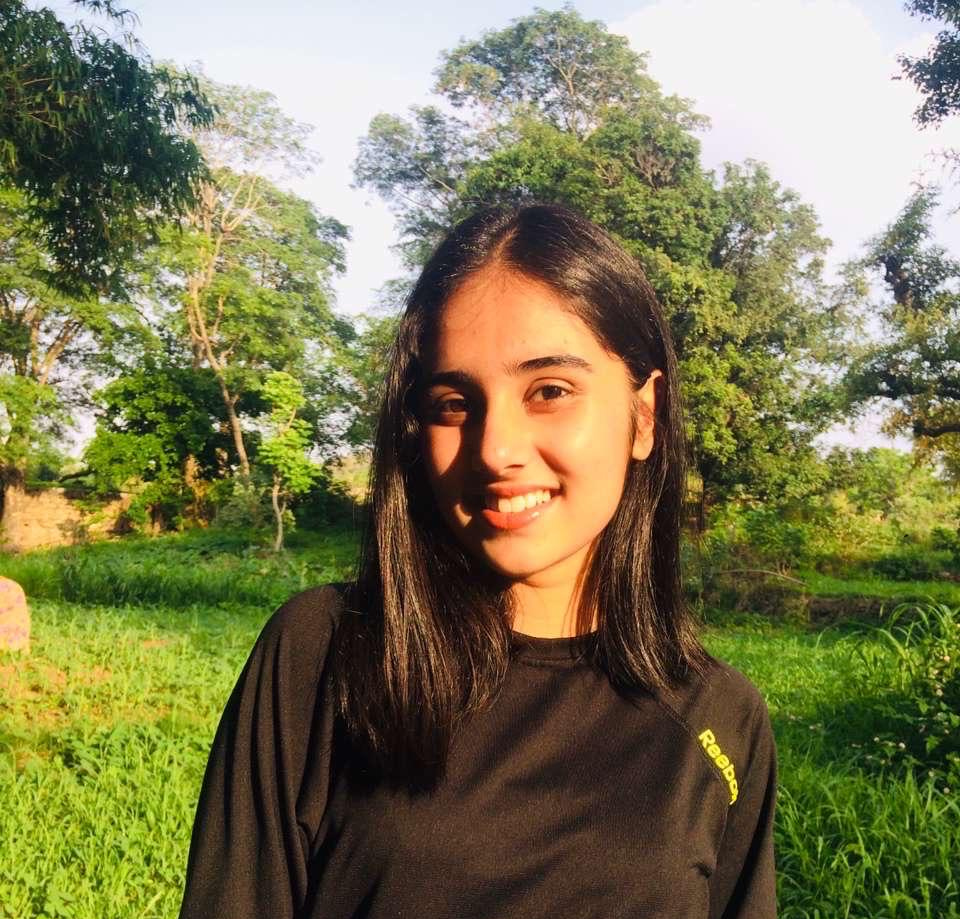
\includegraphics[width=0.4\textwidth]{Assets/SuryanshiRanawat.png}
\end{figure}

\vspace{0.5cm}
\noindent\textbf{Location:} Udaipur \hfill \textbf{Contact:} 6377722486 \\
\textbf{Email:} \href{mailto:suryanshi.23bce11634@vitbhopal.ac.in}{suryanshi.23bce11634@vitbhopal.ac.in} \\
\textbf{Languages:} English, Hindi

\vspace{0.5cm}
\noindent I am currently pursuing a B.Tech in Computer Science and Engineering. I have a strong interest in Artificial Intelligence, Machine Learning, and data-driven problem solving. I have worked on projects such as an AI Disease Detection Platform and a Crop Disease Detection System, which focus on applying AI and machine learning techniques to solve real-world problems in healthcare and agriculture.

\vspace{0.3cm}
\noindent My areas of interest include Artificial Intelligence, deep learning, predictive modeling, and intelligent automation systems. I am particularly interested in exploring how AI can be used to build innovative solutions that improve healthcare, agriculture, and decision-making systems.

% --- UJJWAL MISHRA ---
\newpage
\subsection*{Ujjwal Mishra}
\begin{figure}[H]
  \centering
  
\includegraphics[width=0.4\textwidth]{Assets/UjjwalMishra.png}
\end{figure}

\vspace{0.5cm}
\noindent\textbf{Location:} Delhi \hfill \textbf{Contact:} 8920153120 \\
\textbf{Email:} \href{mailto:ujjwal.23bec10079@vitbhopal.ac.in}{ujjwal.23bec10079@vitbhopal.ac.in} \\
\textbf{Languages:} English, Hindi

\vspace{0.5cm}
\noindent I am currently pursuing a B.Tech in Electronics and Communication Engineering (ECE). I have a strong interest in electronics systems, embedded technologies, and communication networks. I have worked on projects such as a Mobile Network Jammer and a Hexa-Octal Firefighting Drone, which focus on applying engineering concepts to develop practical solutions for safety and communication-related challenges.

\vspace{0.3cm}
\noindent My areas of interest include embedded systems, wireless communication, robotics, and intelligent electronic systems.

\vspace{0.3cm}
\noindent In addition to my technical interests, I possess keen leadership abilities and strong teamwork skills, which help me effectively collaborate and manage project responsibilities. My goal is to continue developing advanced technological solutions that contribute to innovation, safety, and efficient communication systems.

% --- MEDHANSH SINGH KUSHWAHA ---
\newpage
\subsection*{Medhansh Singh Kushwaha}
\begin{figure}[H]
  \centering
  
\includegraphics[width=0.4\textwidth]{Assets/MedhanshSinghKushwaha.png}
\end{figure}

\vspace{0.5cm}
\noindent\textbf{Location:} Agra \hfill \textbf{Contact:} 7055333362 \\
\textbf{Email:} \href{mailto:medhansh.23bce11385@vitbhopal.ac.in}{medhansh.23bce11385@vitbhopal.ac.in} \\
\textbf{Languages:} English, Hindi

\vspace{0.5cm}
\noindent I am currently pursuing a B.Tech in Computer Science Engineering (CSE) with a strong interest in web development, full stack technologies, and digital design. I have experience working with HTML, CSS, React.js, Node.js, and MySQL to build responsive and user-friendly web applications.

\vspace{0.3cm}
\noindent I am also interested in graphic design and UI/UX, using tools such as Adobe Photoshop, Figma, and Blender to create visual content and interface designs. Currently, I am contributing to a Breast Cancer Detection project, where I apply my development and design skills to support the software and interface aspects of the system.

\vspace{0.3cm}
\noindent Along with my technical skills, I possess strong creativity, problem-solving ability, and teamwork skills, and I aim to develop innovative technology solutions that contribute to meaningful real-world applications.

% --- SOUMYADEEP CHAKRAVARTI ---
\newpage
\subsection*{Soumyadeep Chakravarti}
\begin{figure}[H]
  \centering
  
\includegraphics[width=0.4\textwidth]{Assets/SoumyadeepChakravarti.png}
\end{figure}

\vspace{0.5cm}
\noindent\textbf{Location:} Delhi \hfill \textbf{Contact:} 9599059229 \\
\textbf{Email:} \href{mailto:soumyadeep.23bai11250@vitbhopal.ac.in}{soumyadeep.23bai11250@vitbhopal.ac.in} \\
\textbf{Languages:} English, Hindi

\vspace{0.5cm}
\noindent I am currently pursuing a B.Tech in Computer Science and Engineering with a specialization in Artificial Intelligence. I have a strong interest in Artificial Intelligence, Machine Learning, and systems programming. I have worked on projects such as Jarvis, a C-based AI personal assistant that integrates local language models for intelligent interaction, and PyProbe, a tool for exploring Python's internal memory structures and object layouts.

\vspace{0.3cm}
\noindent My areas of interest include Artificial Intelligence, deep learning, and systems-level software development. I am particularly interested in exploring how AI can be combined with efficient low-level programming to build intelligent assistants, advanced tooling, and scalable AI systems.

\end{document}
